%!TEX TS-program = xelatex
%!TEX encoding = UTF-8 Unicode

\documentclass[a4paper,11pt,twoside]{book}
\usepackage{upatras-thesis}


%
% These commands need to be defined in order to produce a correct and personalised document
%
\newcommand{\shortdoctitle}{Διπλωματική Εργασία}
\newcommand{\doctitle}{Εντοπισμός Ακουστικής Πηγής με Βαθιά Νευρωνικά Δίκτυα 
Χρησιμοποιώντας Αμφιωτικές Παραμέτρους}
\newcommand{\docsubtitle}{Υπότιτλος εγγράφου}
\newcommand{\division}{Τηλεπικοινωνιών και Τεχνολογίας Πληροφορίας (Τ\&ΤΠ)}
\newcommand{\lab}{Ενσύρματης Επικοινωνίας}

\newcommand{\me}{Παναγιώτη Ζάχου του Σωτηρίου} %ΠΡΟΣΟΧΗ: στοιχεία σε γενική πτώση. Παράδειγμα: Άγγελου Σικελιανού του Ιωάννη
%
\newcommand{\nomme}{Παναγιώτης Ζάχος του Σωτηρίου} %ΠΡΟΣΟΧΗ: στοιχεία σε ονομαστική πτώση. Παράδειγμα: Άγγελος Σικελιανός του Ιωάννη
%
\newcommand{\studnum}{1019336}
\newcommand{\keywords}{Αμφιωτικές παράμετροι, Νευρωνικά Δίκτυα, Εκτίμηση DOA, Συμπίεση Δεδομένων}
\newcommand{\monthyear}{Ιούλιος 2020}

\newcommand{\supname}{Ιωάννης Μουρτζόπουλος}
\newcommand{\suptitle}{Καθηγητής}
\newcommand{\headofdivision}{Ιωάννης Μουρτζόπουλος}
\newcommand{\headofdivisiontitle}{Καθηγητής}

\author{\me}


% PDF settings
%
\hypersetup
{
    pdfauthor={\me},
    pdftitle={\shortdoctitle},
    pdfsubject={\doctitle},
    pdfkeywords={\keywords},
    pdfproducer={XeLaTex},
    pdfcreator={\creator}
}

\begin{document}

\pagenumbering{roman}
%set the number of sectioning levels that get number and appear in the contents
\setcounter{page}{3}

\begin{titlepage}
\begin{center}
% Upper part of the page
\textsc{\textbf{\large ΠΑΝΕΠΙΣΤΗΜΙΟ ΠΑΤΡΩΝ - ΠΟΛΥΤΕΧΝΙΚΗ ΣΧΟΛΗ}\\
\large ΤΜΗΜΑ ΗΛΕΚΤΡΟΛΟΓΩΝ ΜΗΧΑΝΙΚΩΝ\\ΚΑΙ ΤΕΧΝΟΛΟΓΙΑΣ ΥΠΟΛΟΓΙΣΤΩΝ}\\


\includegraphics[width= 0.8\textwidth]{images/up_2017_logo_en.png}\\  

\textsc{\Large τομέας: \division \\
εργαστήριο: \lab }\\[1cm]

\textsc{\uline{\LARGE{\shortdoctitle }}}\\ [0.5cm]
του φοιτητή του Τμήματος Ηλεκτρολόγων Μηχανικών και Τεχνολογίας\\
Υπολογιστών της Πολυτεχνικής Σχολής  του Πανεπιστημίου Πατρών\\[1cm]

\textsc{\LARGE \me }\\[0.5cm]
\textsc{\Large αριθμός μητρώου: \studnum}\\[1cm]

\uline{\large Θέμα}\\[0.5cm]
\textbf{\large \doctitle }\\[1cm]
\uline{\large Επιβλέπων}\\[0.5cm]
\large \suptitle \, \supname \\[1cm]
\large{Αριθμός Διπλωματικής Εργασίας: }\hspace{3cm}
\vfill
% Bottom of the page
\large{Πάτρα, \monthyear}
\end{center}
\end{titlepage}
\clearemptydoublepage

\pagestyle{empty}
\begin{center}
{\LARGE ΠΙΣΤΟΠΟΙΗΣΗ\\[1cm]}
\large Πιστοποιείται ότι η διπλωματική εργασία με θέμα\\[1cm]
\textbf{\large \doctitle }\\[1cm]
του φοιτητή του Τμήματος Ηλεκτρολόγων Μηχανικών και Τεχνολογίας Υπολογιστών\\[1.5cm]
\me \\[0.5cm]
(Α.Μ.: \studnum )\\[1.5cm]
παρουσιάτηκε δημόσια και εξετάστηκε στο τμήμα  Ηλεκτρολόγων Μηχανικών και Τεχνολογίας Υπολογιστών στις\\[1cm]
\Large{\_\_/\_\_/\_\_\_}\\[1.5cm]
\end{center}
\begin{minipage}{0.5\textwidth}
\begin{flushleft} \large
Ο Επιβλέπων\\[4cm]
\supname \\
\emph{\suptitle}
\end{flushleft}
\end{minipage}
\begin{minipage}{0.5\textwidth}
\begin{flushright} \large
Ο Διευθυντής του Τομέα\\[4cm]
\headofdivision\\
\emph{\headofdivisiontitle}
\end{flushright}
\end{minipage}
\clearemptydoublepage

\pagestyle{empty}
\begin{center}
\Large{Στοιχεία διπλωματικής εργασίας}\\[1cm]
{\large Θέμα:}
\textbf{\large \doctitle}\\[1cm]
\large {Φοιτητής: \textbf{\nomme}\\[1cm]
\large{Ομάδα επίβλεψης}\\
\textbf{\suptitle \, \supname}\\
% \textbf{Βαθμίδα και Ονοματεπώνυμο Συνεπιβλέποντα}\\
%\textbf{Ονοματεπώνυμο Διδακτορικού Φοιτητή}\\[1cm]
Εργαστήρια\\
\lab \\[1cm]
Περίοδος εκπόνησης της εργασίας:\\ Ιανουάριος 2019 - Ιούλιος 2020\\[1cm]
Η εργασία αυτή γράφτηκε στο \XeLaTeX{} και χρησιμοποιήθηκε η γραμματοσειρά GFS Didot του Greek Font Society.}
\end{center}
\clearemptydoublepage

\pagestyle{plain}
\begin{center}
{\LARGE Περίληψη}\\[1cm]
\end{center}

Στην παρούσα Διπλωματική Εργασία προτείνεται μια νέα μέθοδος συμπίεσης των διαστάσεων των αμφιωτικών παραμέτρων ILD και ITD. Ο στόχος της μεθόδου είναι η βέλτιστη αξιοποίηση αυτών των παραμέτρων για την εκπαίδευση Νευρωνικών Δικτύων καθώς και σε άλλες εφαρμογές μηχανικής μάθησης. Υλοποιούνται επίσης δύο μοντέλα Νευρωνικών Δικτύων, ένα πλήρως διασυνδεδεμένο με δομή που παρομοιάζει έναν πολυεπίπεδο Perceptron, καθώς και ένα CNN, με στόχο την εκτίμηση της γωνίας άφιξης μιας ακουστικής διέγερσης, σε πραγματικά δωμάτια με αντήχηση, από τις συμπιεσμένες παραμέτρους. Τα μοντέλα επιτυγχάνουν εξαιρετική ακρίβεια στην εκτίμηση με το μέσο λάθος να κυμαίνεται κάτω από $5^o$, αξιοποιώντας τις παραμέτρους που έχουν συμπιεστεί κατά έναν παράγοντα $\sim88\%$. Η προσέγγιση εκτίμησης της γωνίας άφιξης σε αυτή την εργασία, ξεπερνά παραδοσιακές μεθόδους εντοπισμού που αξιοποιούν τεχνικές μηχανικής μάθησης, τόσο στον χρόνο που χρειάζεται η εκπαίδευση του μοντέλου, όσο και στα αποτελέσματα που επιτυγχάνονται.

\begin{center}
    \rule{\textwidth}{1pt}
\end{center}{}
\textbf{Λέξεις-κλειδιά:} Αμφιωτικές παράμετροι, Νευρωνικά Δίκτυα, Εκτίμηση 
\\*DOA, Συμπίεση Δεδομένων.
\begin{center}
    \rule{\textwidth}{1pt}
\end{center}{}
\clearemptydoublepage

\begin{center}
{\LARGE Ευχαριστίες}\\[1cm]
\end{center}

Έχοντας πλέον ολοκληρώσει τη διπλωματική μου, θα ήθελα να ευχαριστήσω όλα τα μέλη του Audiogroup για το εξαιρετικό κλίμα συνεργασίας στο εργαστήριο τον τελευταίο χρόνο μου ως προπτυχιακός φοιτητής.

Ιδιαιτέρως θα ήθελα να ευχαριστήσω τον καθηγητή μου κ. Ιωάννη Μουρτζόπουλο, ο οποίος με καθοδήγησε σε κάθε βήμα της εργασίας, δίνοντάς μου κίνητρα να εργάζομαι πάντα για το καλύτερο δυνατό αποτέλεσμα, για όλες τις ευκαιρίες που μου έδωσε να μάθω νέα πράγματα και να εξελιχθώ, και για την εμπιστοσύνη που μου έδειξε καθ' όλη την πορεία της διπλωματικής.

Ευχαριστώ στη συνέχεια τον Γαβριήλ για την προθυμία του να με βοηθήσει σε κάθε πρόβλημα που συναντούσα καθώς και τον Κωνσταντίνο για την καθοδήγησή του.

Ένα μεγάλο ευχαριστώ στην οικογένειά μου, που με στήριξε στις επιλογές μου, σε όλη την πορεία μου ως φοιτητής και σε κάθε εύκολη ή δύσκολη στιγμή.

Τέλος, θέλω να ευχαριστήσω όλους τους κοντινούς ανθρώπους που μου στάθηκαν, ιδιαίτερα τον Μηνά και τον Βασίλη, για όλες τις συζητήσεις και τις όμορφες αναμνήσεις.
\clearemptydoublepage



\tableofcontents
\clearemptydoublepage

\pagenumbering{arabic}
\setcounter{page}{1}

%!TEX root = ../main.tex

\chapter{Εισαγωγή}
\markboth{Εισαγωγη}{}
%\vspace{-1.3in}


\noindent Τα προβλήματα εντοπισμού γωνίας άφιξης (Direction of Arrival - DOA) βασισμένα σε παρατηρήσεις που προκύπτουν από το σήμα που έχει εκπεμφθεί, είναι μια ιδιαίτερα σημαντική λειτουργία της χωρικής ακοής των ανθρώπων. Συνήθως αντιμετωπίζονται με μικροφωνικές διατάξεις, αλλά σε πολλές περιπτώσεις, μόνο δύο μικρόφωνα είναι διαθέσιμα (λ.χ. τοποθετημένα σε ένα τεχνητό ή πραγματικό κεφάλι), το οποίο καθιστά την εκτίμηση της DOA σημαντικά δυσκολότερο πρόβλημα, ιδιαίτερα σε περιβάλλοντα με έντονη αντήχηση, παρόλο που ένας άνθρωπος προσαρμόζεται γρήγορα σε τέτοιες αντίξοες συνθήκες, εντοπίζοντας τους ήχους με έναν εύρωστο τρόπο. Η εκτίμηση της θέσης μιας ακουστικής πηγής, μέσω ενός εκπεμπόμενου ηχητικού σήματος, έχει ευρύ φάσμα εφαρμογών, όπως επόμενης γενιάς εμφυτεύματα κοχλία \cite{Nicoletti2013, Aronoff2010}, ακουστικά βοηθήματα \cite{Grimaldi2019}, ρομπότ \cite{Tahmid2010}, συστήματα κατ' οίκον φροντίδας \cite{Chen2013} και αναγνώρισης ομιλίας \cite{Stern2012}. Ήδη υπάρχουσες στρατηγικές εντοπισμού πηγών, μπορούν να κατηγοριοποιηθούν με έναν ελαστικό τρόπο σε τρεις γενικές κατηγορίες: αυτές που βασίζονται στη μεγιστοποίηση της οδηγούμενης απόκρισης ισχύος (Steered Response Power - SRP) ενός beamformer \cite{Dibiase2001}, τεχνικές που υιοθετούν έννοιες υψηλής φασματικής ανάλυσης \cite{Johnson1993, Haykin1991} και προσεγγίσεις που αξιοποιούν την πληροφορία που προέρχεται από τις διαφορές χρόνων άφιξης (Time Difference of Arrival - TDOA) σε ζεύγη μικροφώνων \cite{Chen2006}. 

Οι περισσότερες μέθοδοι εκτίμησης DOA βασίζονται σε προσεγγίσεις που εντάσονται στην $ 3^\text{η} $ κατηγορία, δηλαδή στην αξιοποίηση του TDOA, με την μέθοδο Generalized Cross-Correlation PHAse Transform (GCC-PHAT) να είναι η επικρατέστερη \cite{Knapp1976}. Μια σύνοψη των τεχνικών TDOA βρίσκεται στο \cite{Chen2006}. Στην πράξη, όλες αυτές οι προσεγγίσεις μπορεί να περιορίζονται από ένα, ή συνδυασμό κάποιων μειονεκτημάτων: υψηλό υπολογιστικό κόστος, μη ρεαλιστικές παραδοχές για τα σήματα ή/και τον θόρυβο, αναξιόπιστη απόδοση σε πραγματικά περιβάλλοντα, ειδικά σε δωμάτια με έντονη αντήχηση. Η αυξημένη διαθεσιμότητα υπολογιστικής δύναμης, έχει επιτρέψει την εμφάνιση νέων μεθόδων, που χρησιμοποιούν αλγορίθμους μηχανικής μάθησης (Machine Learning - ML) που μπορούν να αντιμετωπίσουν το πρόβλημα της εκτίμησης DOA.

Τα συστήματα μηχανικής μάθησης που σχεδιάζονται για αυτό το σκοπό, χρησιμοποιούν διαφορετικά δεδομένα εκπαίδευσης, αρχιτεκτονικές, περιβάλλοντα δοκιμής και μετρικές αξιολόγησης. Η πιο ευρέως διαδεδομένη πλέον μέθοδος, είναι η επιβλεπόμενη μάθηση ή supervised machine learning, η οποία έχει ως στόχο, την εκμάθηση μιας συνάρτησης, ενώ ταυτόχρονα την βελτιστοποιεί, η οποία αντιστοιχίζει μια είσοδο σε μια έξοδο, βασιζόμενη σε παραδείγματα εισόδου-εξόδου που χρησιμοποιούνται κατά την εκπαίδευση. Η συνάρτηση εκτιμάται από labeled δεδομένα εκπαίδευσης, που αποτελούνται από ένα σύνολο παραδειγμάτων εκπαίδευσης \cite{Russel2010, Abadi2015}. Πολλές έρευνες στις οποίες εφαρμόζονται τέτοιες τεχνικές ταξινόμησης DOA και αλγόριθμοι εντοπισμού, έχουν δείξει πως αυτή η προσέγγιση είναι έγκυρη και παρέχει εξαιρετικά αποτελέσματα, πχ χρησιμοποιώντας την στρατηγική random forest ensemble \cite{Kamaris2016, Kamaris2017, Kamaris2018} καθώς και τεχνικές που αξιοποιούν νευρωνικά δίκτυα \cite{Zhang2019, Adavanne2017, Perotin2019}.

Σε αυτή την εργασία γίνεται προσπάθεια να αναπτυχθεί μια νέα προσέγγιση για τη μείωση δεδομένων που προέρχονται από αμφιωτικές παραμέτρους, με κατάλληλο τρόπο για εκτίμηση DOA με regression νευρωνικά δίκτυα. Οι εν λόγω αμφιωτικές παράμετροι, είναι η αμφιωτική διαφορά χρόνου άφιξης και η αμφιωτική διαφορά στάθμης ακουστικής πίεσης (Interaural Time Difference και Interaural Level Difference ITD και ILD αντίστοιχα). Συγκεκριμένα, οι αμφιωτικές παράμετροι προέρχονται από μετρήσεις Binaural Room Impulse Responses (BRIRs) από πραγματικά δωμάτια, όπου τα αντηχητικά αποτελέσματα μεγαλώνουν σημαντικά το μέγεθος του dataset ενώ ταυτόχρονα δεν υπάρχουν αρκετές βάσεις δεδομένων που να πληρούν τις απαιτήσεις που υπήρχαν ως προς την αξιοπιστία, το πλήθος των δεδομένων και την ομοιογένειά τους. Για τον σκοπό αυτό, εκτελέστηκε μια εκτενής συγκριτική μελέτη, κατά την οποία αξιολογήθηκε η απόδοση των νευρωνικών όταν χρησιμοποιήθηκαν οι προτεινόμενες συμπιεσμένες αμφιωτικές παράμετροι και οι ασυμπίεστες για τον ίδιο σκοπό, την εκτίμηση της γωνίας άφιξης. Δοκιμάστηκαν δύο εναλλακτικές αρχιτεκτονικές νευρωνικών: μία πλήρως διασυνδεδεμένη (FC), ουσιαστικά ένας Multilayer Perceptron, και μία συνελικτική (CNN).

Εδώ, οι μέθοδοι που δοκιμάστηκαν, επιχειρούν να προβλέψουν την συνάρτηση από τις μεταβλητές εισόδου, σε συνεχείς πραγματικές μεταβλητές δηλαδή την γωνία άφιξης, από τις αμφιωτικές παραμέτρους που χρησιμοποιούνται ως παραδείγματα εκπαίδευσης. Οι μετρικές που χρησιμοποιήθηκαν για να αξιολογηθεί η απόδοση του εκάστοτε μοντέλου είναι το Μέσο Τετραγωνικό Σφάλμα (Mean Squared Error - MSE), το οποίο χρησιμοποιήθηκε ως εκτιμήτρια συνάρτηση (Objective Function) κατά την εκπαίδευση,  η ρίζα του Μέσου Τετραγωνικού Σφάλματος (Root Mean Squared Error - RMSE) και το Μέσο Απόλυτο Σφάλμα (Mean Absolute Error - MAE) που παρέχουν μια εκτίμηση του πόσο 'μακριά' είναι η προβλεπόμενη DOA, από την πραγματική. 

Όπως έχει αναφερθεί, η μέθοδος συμπίεσης δεδομένων που προτείνεται εδώ, μειώνει δραματικά το πλήθος των διαστάσεων των αμφιωτικών παραμέτρων, επιτυγχάνοντας έναν εντυπωσιακό λόγο συμπίεσης έως και 97\% καθώς και εξαιρετικά αποτελέσματα εκπαίδευσης των Νευρωνικών Δικτύων. Κατ' επέκταση αυτό σημαίνει πως δεν χρειάζεται να γίνει κανένας συμβιβασμός μεταξύ της ταχύτητας σύγκλισης του μοντέλου και της ακρίβειάς του.

Το μεγαλύτερο μέρος της επεξεργασίας των δεδομένων έγινε σε περιβάλλον MATLAB, χρησιμοποιώντας την εργαλειοθήκη Auditory Modeling Toolbox \cite{Soendergaard2013}, ενώ η προεπεξεργασία προτού τα δεδομένα χρησιμοποιηθούν για την εκπαίδευση του Νευρωνικού επεξεργάστηκαν με τη γλώσσα Python, όπου έγινε και η εκπαίδευση χρησιμοποιώντας τη διεπαφή TensorFlow \cite{tensorflow2015-whitepaper}.
\clearemptydoublepage

\chapter{Θεωρία - Μέθοδος}\label{ch:chap2}
%!TEX root = ../main.tex

\noindent 
Στο κεφάλαιο αυτό αναφέρονται οι θεωρητικές έννοιες πάνω στις οποίες στηρίζεται η συγκεκριμένη εργασία. Αρχικά αναλύεται η διαδικασία της στερεοφωνικής και αμφιωτικής ακρόασης, η συνάρτηση μεταφοράς του κεφαλιού καθώς και η έννοια της αμφιωτικής κρουστικής απόκρισης δωματίου. Στη συνέχεια περιγράφονται οι διωτικές παράμετροι, ILD και ITD, καθώς και το μοντέλο του Dietz \cite{Dietz2011} το οποίο εφαρμόστηκε για την εξαγωγή τους και η έννοια του λευκού θορύβου. Στη συνέχεια προσεγγίζονται οι απαραίτητες έννοιες της μηχανικής μάθησης όπως και οι δομές των νευρωνικών που εκπαιδεύτηκαν, τα στοιχεία από τα οποία αυτές αποτελούνται, οι μετρικές αξιολόγησής τους και η σημασία της επιλογής ενός κατάλληλου βελτιστοποιητή (optimizer) στην ταχύτητα σύγκλισης του εκάστοτε μοντέλου.

\section{Στερεοφωνική και Αμφιωτική ακρόαση}

Σε αυτή την ενότητα δίνονται οι βασικές αρχές που διέπουν την αντιληπτική λειτουργία εντοπισμού της θέσης ακουστικών πηγών στο χώρο και οι σχετικές τεχνολογικές προσεγγίσεις που ακολουθούνται από τα ηχητικά συστήματα.

\subsection{Στερεοφωνική ακρόαση}

Ο πλέον διαδεδομένος τρόπος αναπαραγωγής του ήχου για οικιακή ή ατομική ακρόαση είναι η στερεοφωνία που βασίζεται στη χρήση δύο ανεξάρτητων καναλιών (αριστερού-L και δεξιού-R) στα οποία συνδυάζονται πολλαπλά κανάλια και πηγές κατά την ηχογράφηση και τα οποία αναπαράγονται από δύο ηχεία, κατάλληλα τοποθετημένα στο χώρο και σε σχέση με τον ακροατή ή και από ακουστικά κυρίως για ακρόαση από φορητές συσκευές.

Σε ακρόαση με φυσικό τρόπο, η αντίληψη που δημιουργείται από την ύπαρξη μιας ακουστικής πηγής στο ελεύθερο ακουστικό πεδίο ή και χώρο, οφείλεται στα συνδυασμένα ερεθίσματα από τα δύο αυτιά του ακροατή που επιτρέπουν τον προσδιορισμό της θέσης της πηγής. Η λειτουργία του μηχανισμού χωρικής αντίληψης του ήχου στηρίζεται εν πολλοίς στην αποκαλούμενη \textit{\textbf{δυϊκή θεωρία}} (duplex theory). Σύμφωνα με τη θεωρία αυτή, το κάθε αυτί, λόγω της διαφορετικής απόστασής του από την ηχητική πηγή $d_1$ και $d_2$ όπως φαίνεται στο Σχήμα \ref{fig:stereo_listening_mechanism}, λαμβάνει διαφορετικές τιμές ηχητικής πίεσης $p_L(t)$ και $p_R(t)$ λόγω:
\begin{enumerate}
    \item Της εξασθένησης της τιμής της πίεσης συναρτήσει της απόστασης.
    \item Της διαφοράς φάσης ή και σχετικής καθυστέρησης λόγω του διαφορετικού χρόνου άφιξης του ήχου σε κάθε αυτί.
    \item Της πρόσθετης εξασθένησης που δημιουργείται στην ακουστική πίεση στο αυτί που 'καλύπτεται' ακουστικά από το κεφάλι, που δημιουργεί σε περιοχή των συχνοτήτων φαινόμενα ηχητικής σκίασης.
\end{enumerate}{}

Αναλόγως με τη συχνότητα, το ποιος από τους παραπάνω λόγους είναι σημαντικότερος για την εξασθένιση και αναλύεται περαιτέρω στην ενότητα \ref{sec:binaural_cues}, αλλά γενικότερα οι παραπάνω μηχανισμοί λειτουργούν επί το πλείστον συμπληρωματικά.

\begin{figure}[h]
  \centering
  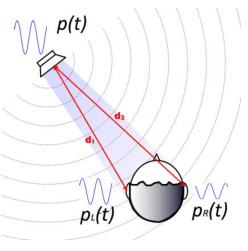
\includegraphics[width=6cm, height=6cm]{images/stereo_listening_mechanism.png}
  \caption{Απεικόνιση του μηχανισμού στερεοφωνικής ακρόασης}
  \label{fig:stereo_listening_mechanism}
\end{figure}

Οι ακροατές εντοπίζουν και διαφοροποιούν με ακρίβεια πηγές που δεν εμφανίζουν σχετικές διαφορές ηχοστάθμης ή/και φάσης στα δύο αυτιά (πχ μια πηγή που είναι ακριβώς μπροστά από το παρατηρητή και μια που είναι ακριβώς από πίσω του στην ίδια απόσταση), στην αντίληψη αξιοποιούνται επιπλέον φαινόμενα ανακλάσεων από τον άνω κορμό (ώμος, στήθος κλπ.) καθώς επίσης και την επίδραση του εξωτερικού πτερυγίου του αυτιού που συλλέγει και διαφοροποιεί τα ηχητικά κύματα που φτάνουν σε αυτό ανάλογα με τις διαφορετικές γωνίες πρόσπτωσης και στα δύο επίπεδα.

\subsection{Αμφιωτική ακρόαση}

Ο άνθρωπος ως ακουστικός δέκτης παρουσιάζει εξαιρετικές ικανότητες στην αναγνώριση και εντοπισμό ηχητικών πηγών στον τρισδιάστατο χώρο. Οι βασικές αρχές αντίληψης της θέσης των πηγών στον τρισδιάστατο χώρο που προαναφέρθηκαν και αφορούν τις σχετικές στάθμες, χρόνους άφιξης ενός σήματος στα 2 αυτιά, της σκίασης του κεφαλιού, της ως προς την γωνία φιλτραρίσματος του σήματος από το πτερύγιο του αυτιού και από τις ανακλάσεις στον άνω κορμό, μπορούν να γενικευθούν σε ένα πλαίσιο που συμπεριλαμβάνει όλους αυτούς τους καθοριστικούς μηχανισμούς και μπορούν να περιγράψουν την αμφιωτική ακρόαση.

Κατά τη γενική περίπτωση αμφιωτικής ακρόασης μιας ακουστικής πηγής, ο ήχος που φτάνει στα δύο αυτιά του ακροατή έχει σαν αποτέλεσμα την αντίληψη και τον προσδιορισμό της θέσης της πηγής σε κάποια γωνία τόσο στο οριζόντιο, όσο και στο κάθετο επίπεδο καθώς και την απόσταση που βρίσκεται αυτή (Σχήμα \ref{fig:binaural_perception_acoustic_source}). Η ικανότητα αυτή προκύπτει από την αντιληπτική διαδικασία που αξιοποιεί τη διαφοροποίηση των σημάτων που φτάνουν στα δύο αυτιά και είναι χαρακτηριστική τόσο για κάθε γωνία στο κάθετο, όσο και στο οριζόντιο επίπεδο. Η δυνατότητα εντοπισμού, εξαρτάται από την μορφολογία του πτερυγίου, του κεφαλιού και του άνω κορμού του εκάστοτε ακροατή. Η ευκρίνεια προσδιορισμού στο οριζόντιο επίπεδο είναι της τάξης των $5^o$ ενώ στο κάθετο επίπεδο είναι αρκετά χειρότερη.

Για την ανάλυση και την περιγραφή της αντιληπτικής διαδικασίας μέσω της δυϊκής θεωρίας, αξιοποιούνται η Αμφιωτική Διαφορά Στάθμης (ILD) και η Αμφιωτική Διαφορά Χρόνου (ITD) που αναλύονται στην ενότητα \ref{sec:binaural_cues}.

Οι δύο αυτές παράμετροι όμως δεν αρκούν για τον προσδιορισμό της θέσης μιας πηγής. Πρέπει να ληφθεί υπόψιν και η διαμόρφωση που εισάγει το εξωτερικό αυτί μέσω του σχήματος του πτερυγίου. Το προσπίπτον σήμα στο κάθε αυτί διαφοροποιείται και φασματικά, αναλόγως με τη γωνία πρόσπτωσης, λόγω της μορφολογίας του πτερυγίου του αυτιού που είναι χαρακτηριστική για κάθε άνθρωπο. Ο τρόπος που το εξωτερικό αυτί συνδυάζεται (μοντελοποιείται) μαζί με τις αμφιωτικές παραμέτρους που αναφέρθηκαν, αναλύονται στην ενότητα \ref{sec:HRTF}


\begin{figure}[h]
  \centering
  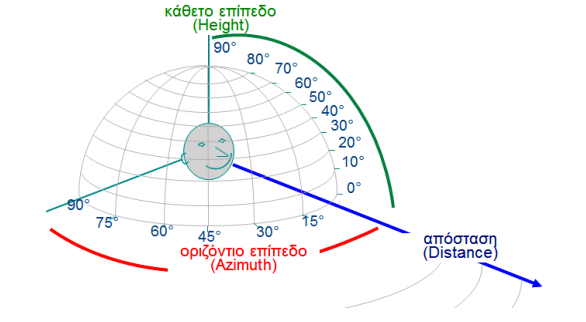
\includegraphics[width=\textwidth]{images/binaural_perception_acoustic_source.png}
  \caption{Αντίληψη και εντοπισμός θέσης πηγής μέσω αμφιωτικής ακρόασης}
  \label{fig:binaural_perception_acoustic_source}
\end{figure}

\section{Συνάρτηση Μεταφοράς Κεφαλιού - HRTF} \label{sec:HRTF}


Η συνάρτηση μεταφοράς του κεφαλιού (Head Related Trasnfer Function - HRTF) είναι μια συνάρτηση μεταφοράς, που για μια συγκεκριμένη γωνία πρόσπτωσης, περιγράφει τη μετάδοση του ήχου από ένα ελεύθερο πεδίο (free field) και την επίδραση του κεφαλιού, του λοβού και του θώρακα σε ένα σημείο στο κανάλι του αυτιού (Σχήμα \ref{fig:auditory_system}) ενός ανθρώπου \cite{mller1995head}. Στο πεδίο του χρόνου η HRTF λέγεται κρουστική απόκριση κεφαλιού (Head Related Impulse Response - HRIR). Η HRIR Παρουσιάζει με έναν εύχρηστο και συνοπτικό τρόπο το ILD και ITD μεταξύ των αυτιών καθώς και άλλες φασματικές πληροφορίες \cite{Enzner2013}.

Στην \cite{doi:10.1121/1.415856}, η συνολική ακουστική μεταφορά από μία ακουστική πηγή σε ελεύθερο χώρο έως το τύμπανο ενός ακροατή, χωρίζεται σε τρία κομμάτια ως εξής:

\begin{itemize}
    \item Μεταφορά από ελεύθερο πεδίο στην φραγμένη είσοδο του ακουστικού καναλιού
    \item Μετατροπή της αντίστασης που σχετίζεται με την φραγή του ακουστικού καναλιού
    \item Μεταφορά μέσω του ακουστικού καναλιού
\end{itemize}{}

\subsection{Μέτρηση HRTF}

Ένα σετ HRTF αριστερού και δεξιού αυτιού εξαρτάται από την θέση της πηγής, την θέση του ακροατή, τη θέση του κεφαλιού και του θώρακα και άλλες παραμέτρους. Οι τυπικές διατάξεις μέτρησης, επιτρέπουν τη μεταβολή ενός ή δύο βαθμών ελευθερίας. Στις περισσότερες περιπτώσεις, μεταβάλλεται η γωνία της πηγής, σε σχέση με το κεφάλι και τον θώρακα που έχουν σταθερό προσανατολισμό. Για την αποτελεσματικότερη μέτρηση HRIR και BRIR (βλ. \ref{sec:BRIR}) έχουν κατασκευαστεί βοηθητικά μοτέρ που επιτρέπουν την περιστροφή ή την αλλαγή της κλίσης του κεφαλιού μέσω λογισμικού, με ακρίβεια μέχρι και $0.01^o$. Συνήθως γίνονται μετρήσεις στο διάστημα $\pm90^o$, με τις $0^ο$ να είναι η πηγή ακριβώς μπροστά από τον δέκτη. Στο Σχήμα \ref{fig:typical-HRTF-measurment-setup} φαίνονται δύο τυπικές διατάξεις μέτρησης HRTF. 

\begin{figure}[h]
  \centering
  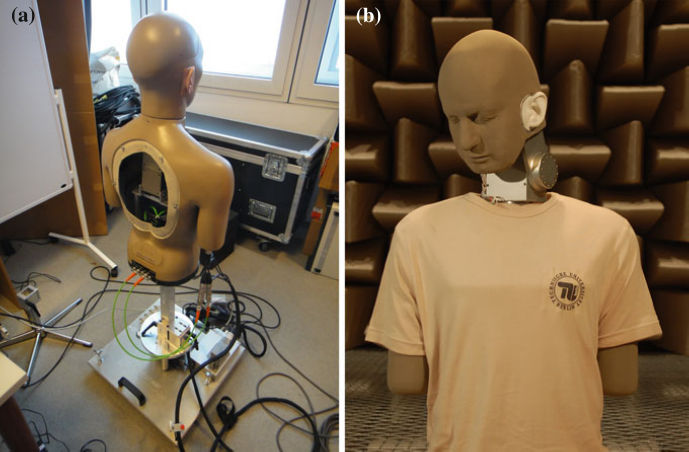
\includegraphics[width=\textwidth]{images/typical-HRTF-measurment-setup.png}
  \caption{Τυπικά σενάρια μέτρησης HRTF: Τροποποιημένο ανδρείκελο KEMAR (a), FABIAN (b)}
  \label{fig:typical-HRTF-measurment-setup}
\end{figure}

\subsection{Υπολογισμός HRTF}

Η επιλογή του σήματος διέγερσης που εκπέμπει η πηγή διαδραματίζει πολύ μεγάλο ρόλο στα αποτελέσματα. Η βέλτιστη διέγερση, εξαρτάται κυρίως από τον αλγόριθμο υπολογισμού της HRIR, αλλά ταυτόχρονα και από το σενάριο μέτρησης (στατικό ή δυναμικό, το περιβάλλον, το υλικό που χρησιμοποιείται κλπ.). Για την επίτευξη ενός υψηλού SNR, το σήμα διέγερσης πρέπει να έχει υψηλή ενέργεια, συγκριτικά με το σύστημα μέτρησης, σε όλη τη συχνοτική περιοχή ενδιαφέροντος. Συχνότερα χρησιμοποιούνται Maximum Length Sequences (MLS), τα οποία είναι περιοδικές ακολουθίες bit που δημιουργούνται από καταχωρητές μετατόπισης γραμμικής ανατροφοδότησης (linear-feedback shift registers) ή απεριοδικά sweep.

Στη συνέχεια, το σήμα αναπαράγεται από το ηχείο-πηγή, και γίνεται συγχρονισμένα η καταγραφή της απόκρισης του αριστερού και δεξιού καναλιού. Η απόκριση συχνότητας προκύπτει από γραμμική αποσυνέλιξη, συνήθως στο πεδίο της συχνότητας. Ένα αποδεκτό SNR για τέτοιου είδους μετρήσεις είναι κάπου ανάμεσα στα 60-90 dB. Μετρήσεις HRTF, πλέον γίνονται και σε ανθρώπους, όχι μόνο σε ανδρείκελα, με ειδικά κατασκευασμένα ακουστικά το περίβλημα των οποίων τυπώνεται με 3Δ εκτυπωτές. 

\subsection{Βάσεις δεδομένων HRTF}

Οι HRTF είναι ένα αναπόσπαστο κομμάτι της τεχνολογίας αμφιωτικής ακοής και ακρόασης. Από την άλλη, η μέτρηση των HRTF είναι ένα δύσκολο και ευαίσθητο εργαστηριακό αντικείμενο. Συνήθως απαιτείται ένας ανηχοϊκός θάλαμος για τη μέτρηση των HRTF, και επιπλέον αρκετός χρόνος από την πλευρά του χειριστή του πειράματος αλλά και του υποκειμένου μέτρησης, ώστε να ολοκληρωθούν οι μετρήσεις με ικανοποιητικό βαθμό χωρικής ανάλυσης. Απαιτούνται ένα ή περισσότερα ηχεία, ακουστικά in-ear, και λογισμικό αναπαραγωγής και καταγραφής ήχου. 

Υπάρχουν αρκετά τέτοια συστήματα, αλλά είναι σαφές πως δεν είναι φορητά. Ως αποτέλεσμα, πολλοί οργανισμοί έχουν επιλέξει να παρέχουν τις μετρήσεις ως δημόσια διαθέσιμες βάσεις δεδομένων στην κοινότητα. Παρακάτω αναφέρονται κάποιες από αυτές. Εκτός αν αναφέρεται διαφορετικά, οι κρουστικές αποκρίσεις παρέχονται με συχνότητα δειγματοληψίας $F_s = 44.1 kHz$.

\begin{itemize}
   \item KEMAR - βάση δεδομένων HRTF από το MIT-Media-Lab \cite{Gardner1995}: Η πρώιμη αυτή βάση δεδομένων είναι ακόμα ιδιαίτερα δημοφιλής, χρησιμοποιώντας το Knowles-Electronics Mannequin for Acoustic Research (KEMAR), αναπαριστά μια εκτενή καταγραφή HRTF. Συνολικά, δειγματοληπτούνται 710 διαφορετικές θέσης, για ανύψωση από $-40^o$ μέχρι $+90^o$ με χωρική ανάλυση $10^o$ στον κάθετο άξονα και περίπου $5^o$ στον οριζόντιο, για απόσταση περίπου 1.4 m μεταξύ του ηχείου και του KEMAR.
   
   \item AUDIS - Ο κατάλογος AUDIS ανθρωπίνων HRTF: Στο γενικό πλαίσιο της Ε.Ε., το project Auditory Displays (AUDIS) \cite{Blauert_1998}, το οποίο βασίστηκε σε μεγάλο βαθμό στην αμφιωτική τεχνολογία και αξιόπιστες HRTF ανθρώπων, πραγματοποιήθηκε ένα ειδικό πρόγραμμα συλλογής HRTF. Εδώ οι συνθήκες μετρήσεων είναι: 2.4 m από το ηχείο, ανάλυση $10^o$ στον κάθετο άξονα από $-10^o$ μέχρι $+90^o$, και ανάλυση $15^o$ στον οριζόντιο άξονα. Οι συνολικές μετρήσεις περιλαμβάνουν 122 κατευθύνσεις για 20 ανθρώπους. Τέθηκε επίσης ένα σύνολο \textit{Golden Rules} για μετρήσεις HRTF.
   
   \item CIPIC - βάση δεδομένων HRTF του εργαστηρίου CIPIC \cite{AlgaziOct.21242001}: Η βάση δεδομένων, περιέχει HRTF μετρημένες με υψηλή χωρική ανάλυση, για περισσότερους από 90 ανθρώπους, με 45 αυτών να είναι δημόσια διαθέσιμοι, συμπεριλαμβανομένου του KEMAR, με μεγάλο και μικρό λοβό. Η χωρική ανάλυση είναι $5^o$ στον κάθετο αλλά και στον οριζόντιο άξονα. Προκύπτουν έτσι 1250 σημεία στην ακουστική σφαίρα 1m, όπου ήταν η απόσταση του ηχείου. Παρέχονται επίσης ανθρωπομετρικά χαρακτηριστικά για κάθε υποκείμενο μέτρησης, καθώς και βοηθητικές συναρτήσεις για το περιβάλλον MATLAB.
   
   \item LISTEN - η βάση δεδομένων HRTF IRCAM: Αναπτηγμένη σε πρότζεκτ της Ε.Ε., περιέχει μετρήσεις HRTF με για  ανύψωση από $-45^o$ μέχρι $+90^o$ με χωρική ανάλυση $5^o$ και περίπου $15^o$ ανάλυση στον οριζόντιο άξονα. Συνολικά μετριούνται 187 θέσεις. Παρέχονται οι μετρήσεις HRTF, προαιρετική διόρθωση diffuse-field και μορφολογικά δεδομένα. Τα δεδομένα που μετρήθηκαν για 50 ανθρώπους είναι διαθέσιμα online\footnote{http://recherche.ircam.fr/equipes/salles/listen/index.html}.
   
   \item ARI - Βάση δεδομένων του Acoustics-Research-Institute: Περιέχει HRTF υψηλής ανάλυσης για πάνω από 70 ανθρώπους. Μετρήθηκαν 1550 θέσεις για κάθε ακροατή, με $2.5^o$ ανάλυση στον οριζόντιο άξονα για γωνίες από $0^o - 359^o$, και ανυψώσεις από $-30^o$ έως $+80^o$. Τα δεδομένα μπορούν να βρεθούν στον σύνδεσμο\footnote{http://www.kfs.oeaw.ac.at/content/view/608/606}.
   
   \item FIU - Βάση δεδομένων HRTF του Florida-International-Univ. DSP-Lab: Μετρήθηκαν 15 διαφορετικά άτομα, για δώδεκα διαφορετικές γωνίες στον οριζόντιο άξονα και έξι στον κάθετο. Παρέχονται 3-Δ εικόνες των λοβών κάθε ατόμου, και ανθρωπομετρικά χαρακτηριστικά. Χρησιμοποιήθηκε συχνότητα δειγματοληψίας $F_s = 96 kHz$ και είναι διαθέσιμη στον σύνδεσμο\footnote{http://dsp.eng.fiu.edu/HRTFDB}.
\end{itemize}

\section{Αμφιωτική Κρουστική Απόκριση Δωματίου - BRIR} \label{sec:BRIR}

Όταν ένας ήχος εκπέμπεται από μια πηγή σε έναν κλειστό χώρο, ένας ακροατής αρχικά θα λάβει τον άμεσο ήχο, ακολουθούμενο από ανακλάσεις από τους τοίχους ή αντικείμενα τοποθετημένα μέσα στο δωμάτιο, όπως φαίνεται στο Σχήμα \ref{fig:listener_reverberant_room}. 

\begin{figure}[h]
  \centering
  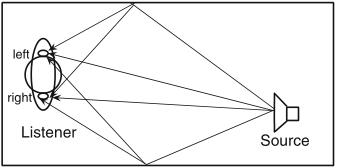
\includegraphics[width=\textwidth]{listener_reverberant_room.png}
  \caption{Ακροατής και ακουστική πηγή σε δωμάτιο με αντήχηση}
  \label{fig:listener_reverberant_room}
\end{figure}

Η ενέργεια του ανακλώμενου ήχου εξασθενεί, σύμφωνα με τα χαρακτηριστικά απορρόφησης των εκάστοτε επιφανειών στο δωμάτιο. Υποθέτοντας ότι η ακουστική του δωματίου, μοντελοποιείται ως ένα \textit{γραμμικό, χρονικά-αμετάβλητο} (ΓΧΑ), σύστημα, η κρουστική απόκριση του δωματίου, (Room Impulse Response - RIR), παρέχει μια πλήρη περιγραφή των άμεσων και ανακλώμενων μονοπατιών από μια πηγή στον δέκτη. Ο χρόνος που χρειάζεται για να ελαττωθεί η ενέργεια του δωματίου κατά 60 dB, αφού η πηγή έχει σταματήσει να εκπέμπει καλείται χρόνος αντήχησης $RT_{60}$ και είναι η παράμετρος που χρησιμοποιείται πιο συχνά για τον προσδιορισμό των ακουστικών ιδιοτήτων ενός δωματίου \cite{Tsilfidis2013}. Σε ένα γενικό, πολυκαναλικό σενάριο, με μία πηγή και \textit{i} δέκτες, το αντιχητικό σήμα $x_i(n)$, μπορεί να εκφραστεί σαν την συνέλιξη του ανηχοϊκού σήματος $s(n)$, με τις αντίστοιχες RIR, $h_i(n)$, ως εξής:

\begin{CEquation}
    x_i(n) = \sum_{j=0}^{J_h - 1} h_i(j)s(n-j) \label{eq 1}
\end{CEquation}

Όπου n αναπαριστά τον δείκτη διακριτού χρόνου και $J_h$ το μήκος της κρουστικής απόκρισης.

Σε ένα αμφιωτικό σενάριο (binaural) η απόκριση του δωματίου, συνδυάζεται με την κρουστική απόκριση του κεφαλιού (Head Related Impulse Response - HRIR), η οποία αποτελείται από δύο κανάλια, ένα για κάθε αυτί. Οι HRIR μετρούνται σε ανηχοϊκές συνθήκες. Συνεπώς, υποθέτοντας μια ιδεατή παντοκατευθυντική πηγή, μία αμφιωτική κρουστική απόκριση δωματίου, για το αριστερό αυτί-κανάλι, $h_L(n)$, μπορεί να εκφραστεί ως

\begin{CEquation}
\begin{split}
    h_L(n) = g(r_s)δ(n-n_s) * h_{\textit{HRIR},L,\theta_d,\phi_d}(n) \\+  \sum_{m=0}^{J_{h_m} - 1} h_{m,L}(n)*h_{\textit{HRIR},L,\theta_m,\phi_m}(n) \label{eq 2}
\end{split}
\end{CEquation}

όπου $g(r_s)$ είναι η ελάτωση του κέρδους που εξαρτάται από την απόσταση πηγής-παρατηρητή $r_s$, $\delta(n)$ η συνάρτηση δέλτα του Kronecker, $n_s$ η καθυστέρηση που εξαρτάται κυρίως από την απόσταση πηγής-παρατηρητή και τα φυσικά χαρακτηριστικά του μέσου διέλευσης. $h_{\textit{HRIR},L,\theta_m,\phi_m}(n)$ είναι η αριστερή HRIR για τον άμεσο ήχο, που αντιστοιχεί σε $\theta_d$ και $\phi_d$, δηλαδή την οριζόντια και κάθετη γωνία μεταξύ του παρατηρητή και της πηγής. Η τιμή $h_m(n)$ αναφέρεται στην m-οστή ανάκλαση. $J_{h_m}$ ο συνολικός αριθμός ανακλάσεων. Τέλος $\theta_m$ and $\phi_m$ είναι οι οριζόντιες και κάθετες γωνίες μεταξύ του δέκτη και της m-οστής ανάκλασης. Αντίστοιχα υπολογίζεται και η BRIR, $h_R(n)$. 

Έτσι, το αντηχητικό σήμα στο αριστερό και δεξί αυτί ενός ακροατή $x_L(n)$ και $x_R(n)$, περιγράφονται με τη συνέλιξη του ανηχοϊκού σήματος $s(n)$, με τις BRIR του αριστερού και δεξιού αυτιού αντίστοιχα, όπως φαίνεται στην Εξίσωση \ref{eq 3}.  Ένα παράδειγμα BRIR από ένα δωμάτιο με ιδιαίτερα υψηλή αντήχηση φαίνεται στο Σχήμα \ref{fig:BRIR_example}

\begin{CEquation}
\begin{split}
    x_L(n) = \sum_{j=0}^{J_{h_L} - 1} h_L(j)s(n-j) \\  \label{eq 3}
    x_R(n) = \sum_{j=0}^{J_{h_R} - 1} h_R(j)s(n-j)
\end{split}
\end{CEquation}

\begin{figure}[H]
  \centering
  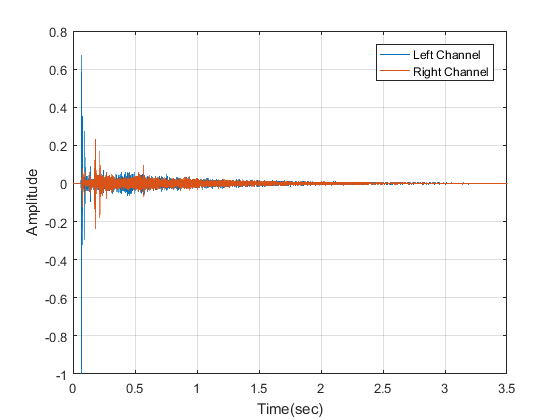
\includegraphics[width=\textwidth]{images/BRIR_example.png}
  \caption{BRIR από δωμάτιο με υψηλή αντίχηση}
  \label{fig:BRIR_example}
\end{figure}

\section{Αμφιωτικές Παράμετροι} \label{sec:binaural_cues}


Το ακουστικό σύστημα, μπορεί να παρομοιαστεί με έναν υπολογιστή πολλαπλών χρήσεων με δύο θύρες εισόδου. Οι θύρες είναι τα δύο αυτιά, στο ίδιο ύψος εκατέρωθεν ενός στερεού ελλειψοειδούς, το κεφάλι.  Το κεφάλι λειτουργεί ως \textit{φορέας μιας κεραίας}, που μπορεί να κινηθεί με έξι βαθμούς ελευθερίας σε σχέση με το σώμα, ενώ το ίδιο το σώμα μπορεί να προηγηθεί στον τρισδιάστατο χώρο, και να αλλάξει τον προσανατολισμό του σε σχέση με τη θέση αναφοράς \cite{Kohlrausch2013}. Μία σύντομη ανατομική περιγραφή του ακουστικού συστήματος φαίνεται στο Σχήμα \ref{fig:auditory_system}

\begin{figure}[h]
  \centering
  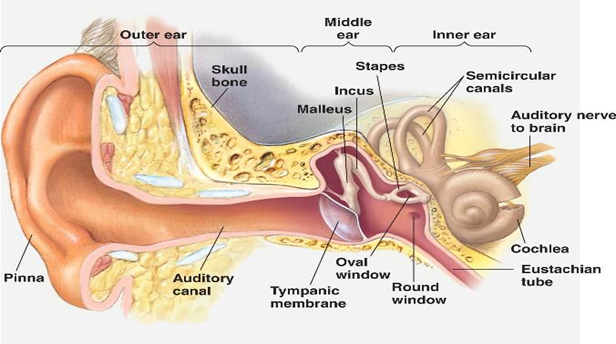
\includegraphics[width=\textwidth]{images/auditory_system.png}
  \caption{Ανατομική περιγραφή του ακουστικού συστήματος}
  \label{fig:auditory_system}
\end{figure}

Το ακουστικό σύστημα δέχεται εισόδους με τη μορφή ελαστικών δονήσεων και κυμάτων, από υγρά ή στερεά με τα οποία είναι σε μηχανική επαφή. Οι είσοδοι έρχονται είτε μέσω του αέρα από τα ακουστικά κανάλια (ear canals) είτε από την μεταβίβαση των οστών μέσω του κρανίου. Συνήθως το κρανίο αγνοείται όταν πρόκειται για ακρόαση σε αέρα, αφού διαφέρει κατά περίπου 60 dB σε σχέση με την μεταβίβαση λόγω αέρα, που αντιστοιχεί σε έναν λόγο ισχύος της τάξεως του $10^6$.

Η ακοή επιτυγχάνεται και με ένα μόνο αυτί, αλλά η ακρόαση με δύο λειτουργικά αυτιά, ή \textit{αμφιωτική ακρόαση}, προσφέρει σημαντικά πλεονεκτήματα έναντι της μονοωτικής ακρόασης. Αυτό, συμβαίνει διότι η αμφιωτική ακρόαση προσφέρει επιπλέον πληροφορία, η οποία κωδικοποιείται στις διαφορές των σημάτων εισόδου στα δύο αυτιά.

Υποθέτοντας ότι αυτές οι διαφορές αναπαρίστανται με ένα γραμμικό, χρονικά αμετάβλητο σύστημα, προκύπτει το συμπέρασμα, ότι μπορούν να υπάρχουν μόνο δύο τέτοιες διαφορές. Η αμφιωτική διαφορά χρόνου άφιξης (Interaural Time Difference - ITD) και οι αμφιωτικές διαφορές έντασης (Interaural Level Difference - ILD). Και οι δύο εξαρτώνται από τη συχνότητα.

Τα υπάρχοντα μοντέλα, αξιοποιούν τις ακουστικές παραμέτρους, που διακρίνονται σε αμφιωτικές παραμέτρους, που είναι πιο εύρωστες και απαιτούν και τα δύο αυτιά για να αναλυθούν, και σε μονοωτικές παραμέτρους που χρειάζονται μόνο το ένα αυτί. Εδώ αναλύονται μόνο οι αμφιωτικές παράμετροι αφού αυτές χρησιμοποιήθηκαν για την προσέγγιση του προβλήματος.

\subsection{Interaural Time Difference}

Παρουσιάζεται πρώτα η ανάλυση του ITD, γιατί ιστορικά το μοντέλο Jefress \cite{Jeffress1948} ήταν το πρώτο μοντέλο εντοπισμού, το 1948. Η βασική ιδέα αυτού του μοντέλου είναι ένας συνδυασμός, \textit{γραμμών καθυστέρησης} και \textit{κυττάρων σύμπτωσης} (coincidence cells). Με βάση το μοντέλο, υπάρχουν δύο ξεχωριστές, παράλληλες γραμμές καθυστέρησης σε κάθε αυτί. Τα σήματα διαδίδονται με αντίθετη κατεύθυνση σε κάθε γραμμή, όπως φαίνεται στο Σχήμα \ref{fig:jeffress-coincidence-mechanism}. Σε κάποιο σημείο, τα σήματα που ταξιδεύουν στις δύο γραμμές, συναντούνται σε ένα κύτταρο σύμπτωσης, το οποίο στέλνει το σήμα στο επόμενο επίπεδο. Λόγω της διαφοράς χρόνου άφιξης των δύο σημάτων στα αυτιά, αυτά θα ενεργοποιήσουν ένα πλευρικά μετατοπισμένο κύτταρο σύμπτωσης, το οποίο κατ' επέκταση αντιστοιχίζεται σε μια πλευρική γωνία άφιξης.

Οι Cherry και Sayers \cite{Cherry1956}, εισήγαγαν τη χρήση της αμφιωτικής ετεροσυσχέτισης, ως μια μέθοδο για την εκτίμηση του ITD η οποία ορίζεται όπως φαίνεται στην Εξίσωση \ref{IACC}. Με την εσωτερική καθυστέρηση να ορίζεται με \textit{τ} και τα αριστερά και δεξιά σήματα πίεσης, $y_l(t)$ και $y_r(t)$. Έχει αποδειχτεί πως αυτό είναι μια καλή προσέγγιση του μοντέλου Jeffress. Το ITD έχει παρατηρηθεί πως δεν παίζει ιδιαίτερο ρόλο στον εντοπισμό πηγών σε συχνότητες μεγαλύτερες των 1500Hz.

\begin{CEquation}
    \psi_{y_{l,r}}(\tau) = \frac{\int_{t=-\infty}^{\infty}y_l(t)y_r(t+\tau)dt}
    {\sqrt{\int_{t=-\infty}^{\infty}y_l^2(t)dt \int_{t=-\infty}^{\infty}y_r^2(t)dt}}
    \label{IACC}
\end{CEquation}

\begin{figure}[h]
  \centering
  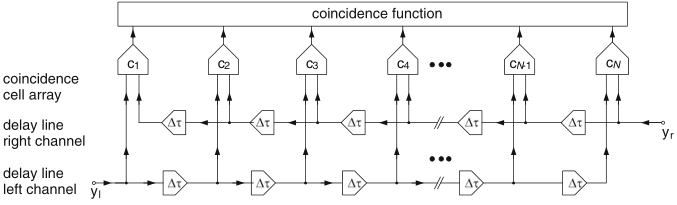
\includegraphics[width=\textwidth]{images/jeffress-coincidence-mechanism.png}
  \caption{Μοντέλο σύμπτωσης όπως αρχικά προτάθηκε από τον Jeffress}
  \label{fig:jeffress-coincidence-mechanism}
\end{figure}

\subsection{Interaural Level Difference}

Οι αμφιωτικές διαφορές έντασης συμβαίνουν λόγω φαινομένων επικάλυψης του κεφαλιού, όταν ένας ήχος φτάνει πλάγια στον δέκτη. Τυπικές τιμές είναι $\pm30 dB$ σε συχνότητες κοντά στα 5 kHz και γωνίες άφιξης στα $\pm60^o$. Στις χαμηλές συχνότητες η επικάλυψη του κεφαλιού δεν παίζει ιδιαίτερο ρόλο, και διαφορές στο ILD σπανίζουν (κάτω από 1500 Hz). Η συχνότητα επικάλυψης ILD και ITD γίνεται φανερό πως είναι στα 1500 Hz.

Το ILD, μπορεί να υπολογιστεί απευθείας από τα σήματα του αριστερού και δεξιού καναλιού όπως φαίνεται στην εξίσωση \ref{ILD_1}, πράγμα το οποίο τυπικά υπολογίζεται για διαφορετικές μπάντες συχνοτήτων, όπου $P_l$ και $P_r$ οι ισχύες των σημάτων που φτάνουν στο αριστερό και δεξί αυτί.
\begin{CEquation}
    \alpha = 10log_{10}(P_l) - 10log_{10}(P_r)
    \label{ILD_1}
\end{CEquation}
Οι Reed και Blum \cite{Reed1990} εισήγαγαν έναν φυσιολογικό (physiological) αλγόριθμο για τον υπολογισμό του ILD, βασισμένο στην δραστηριότητα, $E(\alpha)$, μιας συστοιχίας \textit{El cells}, όπως φαίνεται στο σχήμα \ref{fig:el-cell-structure} και περιγράφεται στην Εξίσωση \ref{eq:reed-and-blum}. Η απόκριση κάθε El-cell είναι συντονισμένη για ένα συγκεκριμένο ILD, και ελατώνεται όσο πιο μακριά από αυτό είναι το ILD των σημάτων άφιξης.

\begin{CEquation}
    E(\alpha) = \exp{
    (10^{\alpha \slash ILD_{max}}\sqrt{P_l} - 
    10^{\alpha \slash ILD_{max}}\sqrt{P_r}})^2
    \label{eq:reed-and-blum}
\end{CEquation}

\begin{figure}[h]
  \centering
  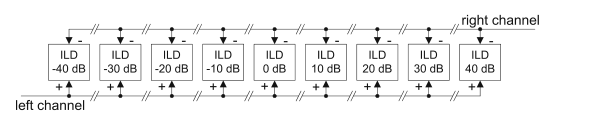
\includegraphics[width=\textwidth]{images/el-cell-structure.png}
  \caption{Δομή El-cell}
  \label{fig:el-cell-structure}
\end{figure}

\subsection{Εντοπισμός ηχητικών γεγονότων}

Υπάρχουν πολλές μέθοδοι για τον υπολογισμό της θέσης ηχητικών πηγών από τις αμφιωτικές παραμέτρους. Μια μέθοδος που επιτυγχάνει αυτόν τον σκοπό, είναι η κατασκευή μια βάσης δεδομένων, που αντιστοιχίζει μετρηθείσες παραμέτρους ILD και ITD σε σφαιρικές συντεταγμένες.

Είναι ακόμα ασαφές πως το ακουστικό σύστημα συνδυάζει τις παραμέτρους για την εξαγωγή συμπερασμάτων για την θέση ακουστικών γεγονότων, συγκεκριμένα, αναπάντητα είναι ακόμα τα εξής ερωτήματα:


\begin{itemize}
    \item Ο τρόπος που συνδυάζονται τα ILD και ITD.
    \item Η ολοκλήρωση της πληροφορίας ως προς τον χρόνο.
    \item Η ολοκλήρωση της πληροφορίας ως προς τη συχνότητα.
    \item Ο διαχωρισμός διαφορετικών, ταυτόχρονων πηγών.
    \item Η αντιμετώπιση των ανακλάσεων του δωματίου.
\end{itemize}

Ότι είναι γνωστό μέχρι στιγμής για τον τρόπο που το ακουστικό σύστημα συνδυάζει τις παραμέτρους έχει προκύψει πειραματικά, από τα αποκαλούμενα trading πειράματα, όπου το ILD υποδεικνύει μια κατεύθυνση, αλλά το ITD μια διαφορετική και ο δέκτης καλείται να κρίνει την πραγματική.

Πιστεύεται ότι το ακουστικό σύστημα, εφαρμόζει χρονικό ή/και συχνοτικό cue weighting, δηλαδή δίνει μεγαλύτερη βαρύτητα σε κάποιες παραμέτρους όταν πληρούνται κάποιες συνθήκες, αλλά ο ακριβής τρόπος που αυτό συμβαίνει είναι ακόμα υπό διερεύνηση. Υπάρχουν διαφορετικές απόψεις, με την μία, που είναι και η επικρατέστερη, να λέει πως το ακουστικό σύστημα δίνει έμφαση στο onset τμήμα του σήματος, ενώ η άλλη να ισχυρίζεται πως ολοκληρώνει την πληροφορία σε μεγαλύτερο χρονικό διάστημα. Τα πράγματα γίνονται σημαντικά δυσκολότερα, όταν δεν είναι σαφές πόσες πηγές υπάρχουν. Τότε οι παράμετροι εκτός από την ανάθεση βαρών σε αυτές, πρέπει να αντιστοιχηθούν και στη σωστή πηγή. Η μεγαλύτερη πρόκληση όμως παραμένει διερεύνηση της αντιμετώπισης των ανακλάσεων του δωματίου από το ακουστικό σύστημα.

\section{Μοντέλο dietz2011} \label{sec:dietz_theory}

Οι Dietz et al. κατασκεύασαν ένα μοντέλο της ανθρώπινης ακοής, με στόχο τον εντοπισμό της κατεύθυνσης ταυτόχρονων ομιλητών στο \cite{Dietz2011}. Ο άνθρωπος έχει μια ιδιαίτερα εύρωστη ικανότητα να εντοπίζει ήχους σε αντίξοες συνθήκες (αντήχηση, έντονος θόρυβος κλπ) οπότε κρίθηκε αναγκαίο να δημιουργηθεί ένα μοντέλο που προσομοιάζει τα χαρακτηριστικά του ανθρώπινου ακουστικού συστήματος με στόχο να χρησιμοποιηθεί αυτό σε αυτόματα συστήματα προσέγγισης DOA.

Η δομή του μοντέλου που κατασκευάστηκε χωρίζεται σε τρία μέρη. Το πρώτο κομμάτι, που θα απασχολήσει αυτή την ενότητα, είναι η ακουστική επεξεργασία για την εξαγωγή των ακουστικών παραμέτρων. Στο δεύτερο, εξάγονται τα σημαντικά τμήματα αυτών των παραμέτρων και στο τρίτο υλοποιείται το σύστημα εντοπισμού. 

\subsection{Ακουστική επεξεργασία}

Εδώ χρησιμοποιήθηκε το μοντέλο ακουστικής επεξεργασίας Interaural Phase Difference \cite{Dietz_2008}, και περιγράφεται παρακάτω.

\begin{enumerate}
    \item Προσεγγίζεται η χαρακτηριστική μεταφοράς του μέσου αυτιού (βλ. \ref{fig:auditory_system}), με ένα πρώτης τάξεως ζωνοπερατό φίλτρο $F_p = 500 Hz, F_c = 2 kHZ$.
    \item Το ακουστικό ζωνοπερατό φιλτράρισμα στην basilar μεμβράνη μοντελοποιείται με μια γραμμική, 4ης τάξης, τράπεζα φίλτρων που αποτελούνται μόνο από πόλους (gammatone filter-bank). Το πλάτος κάθε φίλτρου ορίζεται ως το ισοδύναμο τετραγωνικό εύρως ζώνης (Equivalent Rectangular Bandwidth - ERB) των ακουστικών φίλτρων. Υλοποιούνται 23 μπάντες φίλτρων στο διάστημα των 200 Hz - 5 kHz με απόσταση 1 ERB. Σημειώνεται πως το ERB είναι ένα μέτρο που χρησιμοποιείται στην ψυχοακουστική και δίνει μια εκτίμηση του εύρους ζώνης των φίλτρων στην ανθρώπινη ακοή, χρησιμοποιώντας μη ρεαλιστικά, αλλά βολικά μοντέλα τετραγωνικών ζωνοπερατών φίλτρων.
    \item Η συμπίεση του κοχλία λογιστικοποιήθηκε με άμεση συμπίεση ισχύος 0.4, μετά το bandpass φιλτράρισμα.
    \item Η διαδικασία της ηλεκτρομηχανικής μεταγωγής των εσωτερικών hair-cells, προσομοιώνεται με την ανόρθωση ημίσεος κύματος με διαδοχικά lowpass φίλτρα 5ης τάξης με $F_c = 770 Hz$.
    \item Οι αμφιωτικές χρονικές ανομοιότητες προκύπτουν από το ζωνοπερατό φιλτράρισμα με μιγαδικά gammatone φίλτρα 2ης τάξης.
\end{enumerate}{}

\noindent
Η μιγαδική έξοδος των φίλτρων (Εξίσωση \ref{eq:complex_filter_output}) περιέχει τη διαχωρίσιμη πληροφορία του πλάτους $\alpha(t)$ και της φάσης του σήματος $\phi(t)$.
\begin{CEquation}
    g(t) = \alpha(t) e^{i\phi(t)} \label{eq:complex_filter_output}
\end{CEquation}
Από τα αντίστοιχα αριστερά-δεξιά ζεύγη εξόδων των φίλτρων, $g_l$ και $g_r$, υπολογίζεται η αμφιωτική συνάρτηση μεταφοράς (Interaural Transfer Function - ITF) όπως φαίνεται στην Εξίσωση \ref{eq:ITF}.
\begin{CEquation}
    ITF(t) = g_l(t)\overline{g_r}(t) = 
    \alpha_l(t)\alpha_r(t) e^{i(\phi_l(t)-\phi_r(t))}
    \label{eq:ITF}
\end{CEquation}

Η ITF είναι μιγαδική και περιέχει και αυτή, την πληροφορία για τη φάση και για το πλάτος. Είναι άρα ιδανική για τη χρονική εξομάλυνση των αμφιωτικών συναρτήσεων. Η χρονικά εξομαλυμένη IPD εξάγεται στη συνέχεια από την ITF, αφού αυτή φιλτραριστεί από ένα χαμηλοπερατό φίλτρο, όπως φαίνεται στην Εξίσωση \ref{eq:IPD_extraction}
\begin{CEquation}
    IPD(t) = arg([ITF(t)]_{lp})
    \label{eq:IPD_extraction}
\end{CEquation}

Η IPD μπορεί να μετασχηματιστεί σε ITD διαιρώντας το IPD με την μέση άμεση συχνότητα του αριστερού και δεξιού σήματος. Ο τρόπος υπολογισμού της μέσης άμεσης συχνότητας φαίνεται στην Εξίσωση \ref{eq:instant_freq}

\begin{CEquation}
    f_{inst} = \frac{1}{4\pi}(\frac{d\phi_l(t)}{dt} + \frac{d\phi_r(t)}{dt})
    \label{eq:instant_freq}
\end{CEquation}

Τα μιγαδικά φίλτρα επιτρέπουν τον υπολογισμό της ITF και κατ' επέκταση την IPD της λεπτής-δομής (fine structure) ή της περιβάλλουσας (envelope) του σήματος. Το πρώτο επιτυγχάνεται με το κεντράρισμα του φίλτρου στην ίδια συχνότητα με το προηγούμενο ακουστικό φίλτρο. Για την περιβάλλουσα, το φίλτρο κεντράρεται, στη συχνότητα διαμόρφωσης ενδιαφέροντος, κατά προτίμηση, στην έξοδο του ακουστικού φίλτρου υψηλής συχνότητας. Το φίλτρο λεπτής δομής έχει Q-value 3, ενώ τα φίλτρα διαμόρφωσης έχουν Q-value 8.

Το ILD εκφράζεται σε dB, και πολλαπλασιάζεται με τον παράγοντα συμπίεσης c, όπου $c\sim0.4$ ,όπως φαίνεται στην εξίσωση \ref{eq:ILD_calc} ώστε να κλιμακωθεί η εσωτερική αναπαράσταση στο προτώτυπο ILD, που συμβαίνει στα αυτιά, πριν τη συμπίεση της basilar μεμβράνης.

\begin{CEquation}
    ILD(t) = 20clog_{10}(\frac{|h_r(t)|}{|h_l(t)|})
    \label{eq:ILD_calc}
\end{CEquation}

Το πλεονέκτημα αυτού του μοντέλου είναι η υψηλή φασματική ανάλυση των αμφιωτικών παραμέτρων, που μπορούν να υπολογιστούν δείγμα προς δείγμα. Ακόμα ένα πλεονέκτημα είναι το επιπλέον gammatone φιλτράρισμα που ακολουθεί το μοντέλο ηλεκτρομηχανικής μεταγωγής. Στα κανάλια χαμηλής συχνότητας (περίπου στο 1.4 kHz) ο βασικός λόγος ύπαρξης αυτών των φίλτρων είναι ο διαχωρισμός της DC συνιστώσας από την χρονική λεπτή δομή, όπως απαιτείται από τον υπολογισμό της φάσης. Στα κανάλια υψηλών συχνοτήτων, μπορούν να εφαρμοστούν παράλληλα φίλτρα με τη μορφή μιας τράπεζας φίλτρων διαμόρφωσης ή να προσαρμοστούν στην θεμελιώδη συχνότητα ή στον τόνο ενός συγκεκριμένου ομιλητή. Συνοπτικά το μοντέλο παρουσιάζεται στο Σχήμα \ref{fig:dietz_model_structure}

\begin{figure}[h]
  \centering
  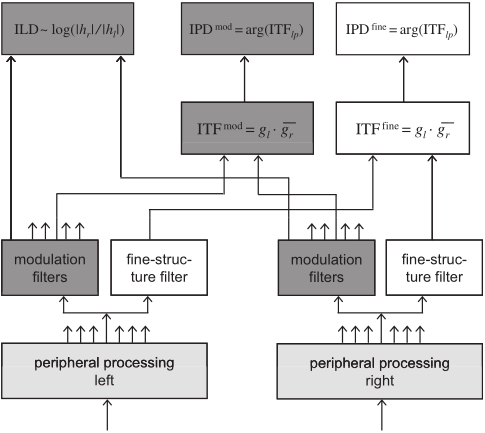
\includegraphics[width=\textwidth]{images/dietz_model_structure.png}
  \caption{Τα στάδια επεξεργασίας του ακουστικού μοντέλου. Η περιφερική επεξεργασία χωρίζει το σήμα εισόδου σε 23 ακουστικά φίλτρα ανά αυτί, και ακολουθείται από ανόρθωση ημίσεος κύματος, χαμηλοπερατό φιλτράρισμα και συμπίεση.}
  \label{fig:dietz_model_structure}
\end{figure}

\section{Λευκός Θόρυβος} \label{sec:white_noise}

Στην επεξεργασία σημάτων ο λευκός θόρυβος, είναι ένα τυχαίο σήμα, που έχει σταθερή ένταση σε όλες τις συχνότητες, δηλαδή σταθερή πυκνότητα φάσματος ισχύος \cite{Carter2009}. Ο όρος χρησιμοποιείται σε διάφορους τομείς, όπως η φυσική, οι τηλεπικοινωνίες και η ακουστική. Στον διακριτό χρόνο, ο λευκός θόρυβος είναι ένα διακριτό σήμα, του οποίου τα δείγματα αντιμετωπίζονται ως μία σειρά ασυσχέτιστων τυχαίων μεταβλητών, με μέση τιμή μηδέν, και πεπερασμένη απόκλιση. Εφόσον ο λευκός θόρυβος ακολουθεί την κατανομή που περιγράφεται στην εξίσωση \ref{eq 4}, αποκαλείται Additive White Gaussian Noise (AWGN). Αξίζει να σημειωθεί πως ο λευκός θόρυβος είναι μια καθαρά θεωρητική κατασκευή, από την άποψη ότι δεν υφίστανται σήματα με άπειρο εύρος ζώνης. Τυπικά ένα σήμα λευκού θορύβου έχει τη μορφή που φαίνεται στο Σχήμα \ref{fig:typical_white_noise}

\begin{CEquation}
    Z_n \sim N(0,W) \label{eq 4}
\end{CEquation}

\begin{figure}[h]
  \centering
  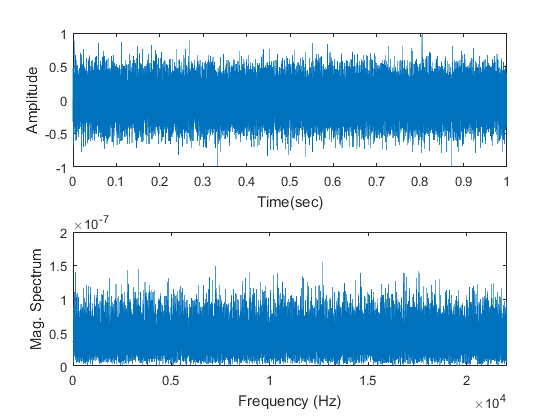
\includegraphics[width=\textwidth, height=8cm]{images/typical_white_noise.png}
  \caption{Τυπική μορφή σήματος λευκού θορύβου, στον χρόνο (Πάνω) και στη συχνότητα (Κάτω)}
  \label{fig:typical_white_noise}
\end{figure}

\section{Μηχανική Μάθηση}

Η ιδέα πίσω από τη μάθηση είναι ότι οι αισθήσεις δεν πρέπει να χρησιμοποιούνται απλώς για άμεση δράση, αλλά και για τη βελτίωση της ικανότητας ενός πράκτορα να ενεργεί στο μέλλον. Πράκτορας είναι οτιδήποτε μπορεί να θεωρηθεί ότι αντιλαμβάνεται το περιβάλλον του μέσω αισθητήρων, και επενεργεί σε αυτό το περιβάλλον μέσω μηχανισμών δράσης (Σχήμα \ref{fig:agent_environment_interaction}). Η μάθηση μπορεί να κυμαίνεται από την απλή απομνημόνευση των εμπειριών, μέχρι τη δημιουργία ολόκληρων επιστημονικών θεωριών. Εδώ περιγράφεται η επαγωγική μάθηση, κατά την οποία ένα σύστημα βελτιώνεται μέσω παρατηρήσεων \cite{Russell1994ArtificialIA}.

\begin{figure}[h]
  \centering
  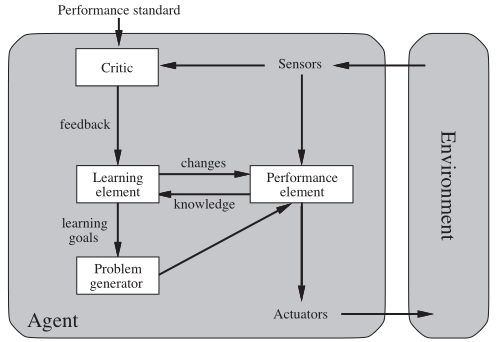
\includegraphics[width=\textwidth]{images/agent_environment_interaction.png}
  \caption{Αλληλεπίδραση πράκτορα με το περιβάλλον του}
  \label{fig:agent_environment_interaction}
\end{figure}

Ένας πράκτορας μπορεί να θεωρηθεί ότι περιλαμβάνει ένα στοιχείο εκτέλεσης, το οποίο αποφασίζει τι ενέργειες θα πραγματοποιήσει, και ένα στοιχείο μάθησης που τροποποιεί το στοιχείο εκτέλεσης έτσι ώστε να λαμβάνει καλύτερες αποφάσεις. Οι ερευνητές της μηχανικής μάθησης έχουν ανακαλύψει μια μεγάλη ποικιλία στοιχείων μάθησης. Για να γίνουν αυτά κατανοητά, είναι χρήσιμο να αποσαφηνιστεί το με ποιον τρόπο η σχεδίασή τους επηρεάζεται από το περιβάλλον στο οποίο θα εφαρμοστούν. Η σχεδίαση ενός στοιχείου μάθησης επηρεάζεται από τρία κύρια ζητήματα:
\begin{itemize}
    \item Ποιες συνιστώσες του στοιχείου εκτέλεσης πρέπει να μαθευτούν.
    \item Τι ανάδραση διατίθεται για τη μάθηση αυτών των συνιστωσών.
    \item Ποια αναπαράσταση χρησιμοποιείται για τις συνιστώσες.
\end{itemize}{}

Συνοπτικά \textbf{στοιχείο εκτέλεσης} είναι το στοιχείο του πράκτορα που είναι υπεύθυνο για εξωτερικές πράξεις και \textbf{στοιχείο μάθησης} το στοιχείο που είναι υπεύθυνο για την υλοποίηση βελτιώσεων στο σύστημα.

Ο \textit{τύπος της ανάδρασης} που διατίθεται για τη μάθηση είναι συνήθως ο πιο σημαντικός παράγοντας για τον προσδιορισμό της φύσης του μαθησιακού προβλήματος. Διακρίνονται τρεις περιπτώσεις: \textbf{μη επιβλεπόμενη μάθηση} (unsupervised learning), \textbf{επιβλεπόμενη μάθηση} (supervised learning) και \textbf{ενισχυτική μάθηση} (reinforcement learning).

\subsection{Μη επιβλεπόμενη μάθηση}
Το πρόβλημα της μη επιβλεπόμενης μάθησης περιλαμβάνει τη μάθηση προτύπων εισόδου χωρίς να παρέχονται συγκεκριμένες τιμές εξόδου. Δύο βασικές μέθοδοι είναι η \textit{ανάλυση σε κύριες συνιστώσες} (Principal Component Analysis - PCA) και η \textit{ανάλυση συστάδων} (cluster analysis). Χρησιμοποιείται ευρέως στην εκτίμηση πυκνοτήτων πιθανοτήτων (pdf) στη στατιστική.

\subsection{Ενισχυτική μάθηση}
Η ενισχυτική μάθηση είναι ένα πεδίο της μηχανικής μάθησης που ασχολείται με τον τρόπο που πράκτορες λογισμικού πρέπει να πάρουν αποφάσεις και να τις εκτελέσουν σε ένα περιβάλλον ώστε να μεγιστοποιήσουν κάποια ανταμοιβή. Όπως και η μη επιβλεπόμενη μάθηση, δεν χρειάζεται συγκεκριμένες τιμές εξόδου. Υλοποιείται τυπικά με την μορφή αλυσίδων αποφάσεων Markov

\subsection{Επιβλεπόμενη μάθηση}
H επιβλεπόμενη μάθηση είναι η διαδικασία της χαρτογράφησης μιας εισόδου σε μία έξοδο, με βάση \textit{labeled} δεδομένων εισόδου, που αποτελούνται από παραδείγματα εισόδου-εξόδου. Με αυτόν τον τρόπο, εκτιμάται μια συνάρτηση με βάση αυτά τα ζεύγη παραδειγμάτων. Κάθε παράδειγμα, είναι ένα ζεύγος, που αποτελείται από ένα αντικείμενο εισόδου, τυπικά ένα διάνυσμα, και μια επιθυμητή τιμή εξόδου. Σε ένα ιδανικό σενάριο, ο αλγόριθμος θα μπορεί να εκτιμήσει σωστά την επιθυμητή έξοδο από περιπτώσεις που δεν έχουν χρησιμοποιηθεί κατά την εκπαίδευση. Σε αυτή την κατηγορία αλγορίθμων μάθησης, εντάσσονται και τα Νευρωνικά Δίκτυα που θα απασχολήσουν αυτή την εργασία.

Πιο αυστηρά, ο στόχος της επιβλεπόμενης μάθησης είναι: Δοθέντος ενός \textbf{συνόλου εκπαίδευσης} Ν παραδειγμάτων ζευγών εισόδου-εξόδου: $$(x_1,y_1), (x_2,y_2), ... (x_N,y_N)$$ όπου κάθε $y_i$ δημιουργείται από μια άγνωστη συνάρτηση $y=f(x)$, να βρεθεί μια συνάρτηση $h$ που προσεγγίζει την $f$.

Όταν η έξοδος $y$ ανήκει σε ένα σύνολο πεπερασμένων τιμών, (λ.χ. ναι, όχι, ίσως) το πρόβλημα μάθησης λέγεται \textbf{ταξινόμηση} (classification). Όταν το $y$ είναι ένας πραγματικός αριθμός, το πρόβλημα λέγεται \textbf{regression}.

\begin{figure}[h]
  \centering
  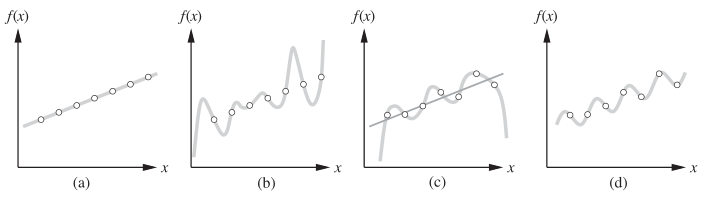
\includegraphics[width=\textwidth]{images/supervised_example_linear.png}
  \caption{Παραδείγματα ζευγών $(x,f(x))$ και υποθέσεις διαφορετικών βαθμών πολυωνύμου (a) 1ου βαθμού, (b) 7ου βαθμού. (c) Ένα διαφορετικό dataset και μια γραμμική εκτίμηση, (d) ημιτονοειδής εκτίμηση}
  \label{fig:supervised_example_linear}
\end{figure}

Στο Σχήμα \ref{fig:supervised_example_linear} φαίνεται ένα σύνηθες παράδειγμα, η προσαρμογή μιας καμπύλης σε ένα σύνολο ζευγών σημείων. Δεν είναι γνωστό ποια είναι η $f$ αλλά προσεγγίζεται με μια \textit{h} επιλεγμένη από τον χώρο υποθέσεων $\mathcal{H}$. Στο παράδειγμα αυτό είναι ένα σύνολο πολυωνύμων. 

Η επιβλεπόμενη μάθηση μπορεί να υλοποιηθεί επιλέγοντας την υπόθεση $h^*$ που είναι πιθανότερη με βάση τα δεδομένα:
\begin{CEquation}
\begin{split}
     h^* = \argmaxF_{h\subset\mathcal{H}} P(h|data)
     \label{eq:hypothesis_star}
\end{split}
\end{CEquation}


Η Εξίσωση \ref{eq:hypothesis_star} με βάση τον κανόνα του Bayes, μετασχηματίζεται στην Εξίσωση \ref{eq:hypothesis_star_bayes} και μπορεί κανείς να ισχυριστεί πως η εκ των προτέρων πιθανότητα $P(h)$ είναι μεγάλη για ένα πολυώνυμο μικρού βαθμού και χαμηλότερη για ένα πολυώνυμο μεγάλου βαθμού. Γενικότερα επιτρέπονται περίπλοκες ή \textit{παράξενες} προσεγγίσεις μόνο όταν κρίνεται ότι το απαιτούν τα δεδομένα, αλλά αποφεύγεται με τον να τους ανατίθεται χαμηλή πιθανότητα. Γενικά, αξίζει να σημειωθεί πως υπάρχει πάντα ένα tradeoff μεταξύ της εκφραστικότητας ενός χώρου υποθέσεων, και της πολυπλοκότητας της εύρεσης μιας καλής υπόθεσης μέσα σε αυτό το χώρο.

\begin{CEquation}
\begin{split}
     h^* = \argmaxF_{h\subset\mathcal{H}} P(data|h)P(h)
     \label{eq:hypothesis_star_bayes}
\end{split}
\end{CEquation}

\section{Νευρωνικά Δίκτυα}

Νευρωνικά Δίκτυα, ή με τον πιο δόκιμο όρο, Τεχνητά Νευρωνικά Δίκτυα (Artificial Neural Networks - ANN), είναι ένα σύνολο από τεχνητούς νευρώνες ή κόμβους \cite{Hopfield_1982}. Ουσιαστικά είναι υπολογιστικά συστήματα εμπνευσμένα από βιολογικά νευρωνικά δίκτυα που έχουν μελετηθεί σε εγκεφάλους διαφόρων ζώων \cite{Chen_2019}. Τα συστήματα αυτά 'μαθαίνουν' να εκτελούν συγκεκριμένο έργο λαμβάνοντας υπόψιν τους παραδείγματα, συνήθως χωρίς να είναι προγραμματισμένα με συγκεκριμένους κανόνες που αφορούν το εν λόγω έργο. Εκτελούν το έργο που τους ανατίθεται, χωρίς να έχουν πρότερη γνώση επί αυτού. 

\subsection{Νευρώνες} 

Ένα ANN βασίζεται σε μια συλλογή νευρώνων οι οποίοι μοντελοποιούν τους νευρώνες ενός βιολογικού εγκεφάλου. Κάθε σύνδεση, όπως οι συνάψεις στον εγκέφαλο, μπορεί να μεταδόσει σήματα στους άλλους νευρώνες. Ένας τεχνητός νευρώνας δέχεται το σήμα, το επεξεργάζεται και στη συνέχεια μεταβιβάζει το επεξεργασμένο σήμα στους νευρώνες με τους οποίους συνδέεται.

Αυστηρότερα, ένας νευρώνας είναι μια \textit{συνάρτηση}, και αποτελεί το δομικό στοιχείο ενός ANN. Δέχεται μία ή περισσότερες εισόδους, (που αντιπροσωπεύουν τα διεγερτικά μετασυναπτικά δυναμικά και τα ανασταλτικά μετασυναπτικά δυναμικά στους δενδρίτες των νευρώνων) τις προσθέτει και μεταδίδει μια έξοδο, (ή ενεργοποίηση που αντιπροσωπεύει το δυναμικό δράσης ενός βιολογικού νευρώνα που μεταδίδεται κατά μήκος του άξονά του). Η αντιστοίχηση φαίνεται στο Σχήμα \ref{fig:biological_neuron_artificial_neuron_cmp}. Συνήθως σε κάθε είσοδο ανατίθεται ένα βάρος και το άθροισμά τους δίνεται ως είσοδος σε μια μη γραμμική συνάρτηση που αποκαλείται \textbf{\textit{συνάρτηση ενεργοποίησης}} ή \textit{συνάρτηση μεταφοράς} του νευρώνα.

\begin{figure}[h]
  \centering
  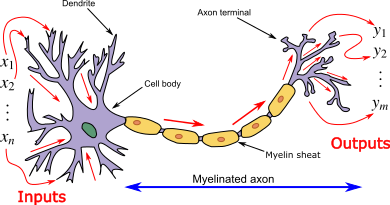
\includegraphics[width=\textwidth]{images/Neuron3.png}
  \caption{Νευρώνας και μυελινωμένος άξονας, με τη ροή του σήματος από τις εισόδους στους δενδρίτες στις εξόδους στον άξονα.}
  \label{fig:biological_neuron_artificial_neuron_cmp}
\end{figure}

\subsubsection{Βασική Δομή Νευρώνα}

Για έναν τεχνητό νευρώνα, έστω \textit{m + 1} είσοδοι με σήματα από $x_0$ μέχρι $x_m$. Η είσοδος σε έναν νευρώνα \textit{k} φαίνεται στην εξίσωση \ref{eq:kth_neuron_input}, όπου με \textit{φ} συμβολίζεται η συνάρτηση μεταφοράς ενώ η δομή ενός νευρώνα φαίνεται στο Σχήμα \ref{fig:artificial_neuron_math_model}.

\begin{CEquation}
\begin{split}
     y_k = \phi(\sum_{j=0}^mw_{kj}x_j)
     \label{eq:kth_neuron_input}
\end{split}
\end{CEquation}

\begin{figure}[h]
  \centering
  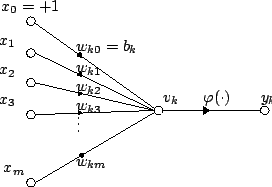
\includegraphics[width=8cm, height=6cm]{images/Artificial_neuron.png}
  \caption{Μαθηματικό μοντέλο ενός νευρώνα με bias στο $x_0 = 1$}
  \label{fig:artificial_neuron_math_model}
\end{figure}

\subsubsection{Συναρτήσεις ενεργοποίησης}

\begin{itemize}
    \item \textbf{Βηματική Συνάρτηση}: Η έξοδος αυτής της συνάρτησης είναι δυαδική και εξαρτάται από το αν η είσοδος ξεπερνά ή είναι ίση με ένα ορισμένο κατώφλι \textit{θ}. Εκτελεί μια διαίρεση του χώρου εισόδων με ένα υπερεπίπεδο. Είναι ιδιαίτερα χρήσιμη όταν εφαρμόζεται στο τελευταίο επίπεδο ενός ANN, που κάνει δυαδική συσταδοποίηση.
    \begin{CEquation}
    \begin{split}
         y = 
         \begin{cases}
         1 & \text{if}\;x\geq\theta\\
         0 & \text{if}\;x<\theta
         \end{cases}   
         \label{eq:step_function}
    \end{split}
    \end{CEquation}
    
    \item \textbf{Σιγμοειδής}: Μια μη-γραμμική συνάρτηση με παράγωγο που υπολογίζεται εύκολα, και κατ' επέκταση είναι υπολογιστικά απλή. Ένα παράδειγμα είναι η γνωστή logistic function:
    \begin{CEquation}
    \begin{split}
         y = \frac{e^x}{e^x + 1}  
         \label{eq:logistic_function}
    \end{split}
    \end{CEquation}
    
    \item \textbf{Συνάρτηση Ανόρθωσης}: Οι συναρτήσεις αυτές είναι γνωστές και ως συναρτήσεις ράμπας, και είναι το υπολογιστικό ανάλογο ενός ανορθωτή ημίσεος κύματος. Λέγονται επίσης Rectified Linear Units ή ReLU και ορίζονται ως εξής:
    \begin{CEquation}
    \begin{split}
         y = x^+ = \max{(0,x)}
         \label{eq:ReLU}
    \end{split}
    \end{CEquation}
    
\end{itemize}{}

\subsection{Οργάνωση}

Οι νευρώνες τυπικά είναι οργανωμένοι σε πολλά επίπεδα, ιδιαίτερα στην περίπτωση του deep learning. Το επίπεδο που δέχεται τα δεδομένα είναι το \textit{επίπεδο εισόδου}, ενώ το επίπεδο που δίνει το τελικό αποτέλεσμα είναι το \textit{επίπεδο εξόδου}. Μεταξύ τους μπορεί να υπάρχουν μηδέν ή περισσότερα \textit{κρυφά επίπεδα}. Τα επίπεδα μπορεί να είναι συνδεδεμένα με πολλούς τρόπους. Για παράδειγμα μπορεί να είναι \textit{πλήρως διασυνδεδεμένα}, με κάθε νευρώνα σε ένα επίπεδο να συνδέεται με όλους τους νευρώνες του επόμενου επιπέδου.

\subsubsection{Υπερπαράμετροι} \label{subsub:hyperparameters}

Μια υπερπαράμετρος είναι μια σταθερή παράμετρος της οποίας η τιμή ορίζεται πριν την εκκίνηση της διαδικασίας εκπαίδευσης. Τέτοιες παράμετροι είναι ο ρυθμός μάθησης (learning rate - LR), ή ο αριθμός των κρυφών επιπέδων.

\subsubsection{Backpropagation}

Το backpropagation είναι μια μέθοδος ρύθμισης των βαρών των συνάψεων για την διόρθωση των σφαλμάτων κατά την εκπαίδευση. Το σφάλμα πρακτικά 'μοιράζεται' σε όλες τις συνάψεις. Υπολογίζονται οι παράγωγοι των συναρτήσεων ενεργοποίησης ανάλογα με τα τωρινά βάρη, και ενημερώνονται αναλόγως με την μέθοδο βελτιστοποίησης που έχει επιλεχθεί. Σε αυτή την εργασία όλα τα μοντέλα χρησιμοποιούν τον Adam optimizer.

\subsubsection{Αρχιτεκτονικές}

Μία από τις αρχιτεκτονικές που χρησιμοποιείται σε αυτή την εργασία είναι ο πολυεπίπεδος Perceptron (Multilayered Perceptron - MLP). Η αρχιτεκτονική αυτή αποτελείται από τουλάχιστον τρία επίπεδα, ένα επίπεδο εισόδου, ένα επίπεδο εξόδου και τουλάχιστον ένα κρυφό επίπεδο, όλα πλήρως διασυνδεδεμένα μεταξύ τους. Η απλούστερη δομή (από την άποψη του αριθμού των επιπέδων) ενός MLP φαίνεται στο Σχήμα \ref{fig:multilayer-perceptron}.

\begin{figure}[h]
  \centering
  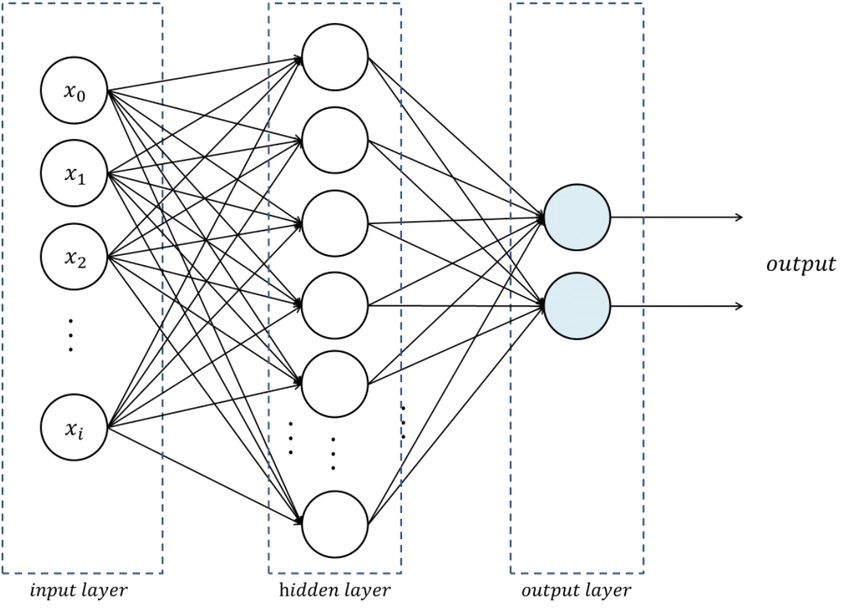
\includegraphics[width=\textwidth]{images/multilayer-perceptron.png}
  \caption{Η δομή του απλούστερου MLP.}
  \label{fig:multilayer-perceptron}
\end{figure}

Η δεύτερη αρχιτεκτονική που χρησιμοποιείται είναι αυτή των συνελικτικών δικτύων (Convolutional Neural Networks - CNNs). Η δομή αυτή είναι αρκετά πιο σύγχρονη από αυτή του MLP, και χρησιμοποιείται συχνά για την ανάλυση εικόνων και προβλήματα που αφορούν την υπολογιστική όραση. Αυστηρά, συνελικτικό δίκτυο είναι κάθε ANN που χρησιμοποιεί την πράξη της συνέλιξης. Στην πράξη, τα CNN, σε αντίθεση με τους MLP αντί να εκτολούν ένα γινόμενο πινάκων, χρησιμοποιούν συνέλιξη. Κάθε συνελικτικό επίπεδο, αποτελείται από έναν αριθμό φίλτρων που ορίζεται προτού ξεκινήσει η εκπαίδευση, όπως και οι διαστάσεις αυτών. Κάθε συνελικτικός νευρώνας επεξεργάζεται μόνο τα δεδομένα που είναι σε μια περιορισμένη υποπεριοχή της εξόδου του προηγούμενου επιπέδου. Μια τυπική δομή ενός CNN φαίνεται στο Σχήμα \ref{fig:convolutional-neural-network-architecture}. Οι λειτουργία των επιπέδων Pooling εξηγείται σε επόμενη ενότητα.

\begin{figure}[h]
  \centering
  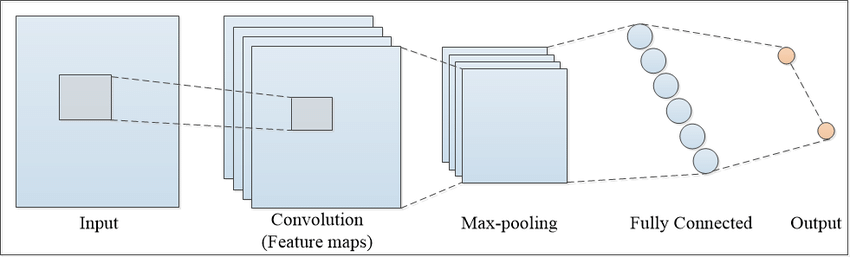
\includegraphics[width=\textwidth]{images/convolutional-neural-network-architecture-showing-a-feed-forward-pass-with-one.png}
  \caption{Η δομή ενός απλού CNN.}
  \label{fig:convolutional-neural-network-architecture}
\end{figure}
\newpage
\subsection{Συναρτήσεις Απώλειας}

Κάθε αλγόριθμος βελτιστοποίησης χρησιμοποιεί μια συνάρτηση για την \textit{αξιολόγηση} μιας πιθανής λύσης (π.χ. το σύνολο των βαρών στις συνάψεις ενός NN). Η συνάρτηση αυτή καλείται αντικειμενική συνάρτηση, και η βέλτιστη λύση είναι αυτή που ελαχιστοποιεί την αντικειμενική συνάρτηση σε προβλήματα ελαχιστοποίησης (ή το αντίθετο σε προβλήματα μεγιστοποίησης) \cite{Goodfellow2017}.

\subsubsection{Μέσο Απόλυτο Σφάλμα}
Το ΜΑΕ, είναι ένα μέτρο της διαφοράς μεταξύ δύο συνεχών μεταβλητών. Υποθέτοντας μεταβλητές Χ και Υ, οι οποίες είναι η πραγματική και η εκτιμώμενη τιμή αντίστοιχα, τότε για \textit{n} παρατηρήσεις το ΜΑΕ υπολογίζεται από την Εξίσωση \ref{eq:MAE}. Το ΜΑΕ έχει τις ίδιες μονάδες με τα δεδομένα που παρατηρούνται και πεδίο ορισμού $D = [0, +\infty)$. 

\begin{CEquation}
\begin{split}
     MAE = \frac{\sum_{i=1}^n|y_i-x_i|}{n}
     \label{eq:MAE}
\end{split}
\end{CEquation}


\subsubsection{Μέσο Τετραγωνικό Σφάλμα}
Το MSE ενός εκτιμητή, υπολογίζει τον μέσο όρο των τετραγώνων των σφαλμάτων, δηλαδή τον μέσο όρο των τετραγώνων των διαφορών της εκτιμώμενης τιμής από την πραγματική. Το MSE, είναι η δεύτερη ροπή (ως προς το 0) του σφάλματος, οπότε περιέχει τόσο την τυπική απόκλιση, δηλαδή το πόσο 'απλωμένες' είναι οι εκτιμήσεις, αλλά και  το \textit{bias}, δηλαδή το πόσο μακριά είναι η μέση εκτιμώμενη από την μέση πραγματική τιμή. Όπως η διακύμανση, έτσι και το MSE, έχει τις μονάδες των δεδομένων παρατήρησης υψωμένες στο τετράγωνο. Χρησιμοποιείται, όταν είναι ιδιαίτερα ανεπιθύμητα μεγάλα σφάλματα στον εκτιμητή, έχει πεδίο ορισμού το $D = [0, +\infty)$, και υπολογίζεται όπως φαίνεται στην εξίσωση \ref{eq:MSE}.

\begin{CEquation}
\begin{split}
     MSE = \frac{\sum_{i=1}^n|y_i-x_i|^2}{n}
     \label{eq:MSE}
\end{split}
\end{CEquation}

\subsubsection{Ρίζα Μέσου Τετραγωνικού Σφάλματος}
Το RMSE, αντιπροσωπεύει την τετραγωνική ρίζα της δεύτερης ροπής των διαφορών μεταξύ των εκτιμώμενων τιμών και των πραγματικών. Όπως και τα προαναφερθέντα μέτρα, είναι θετικά ορισμένο, με πεδίο ορισμού το $D = [0, +\infty)$. Συνδυάζει τα πλεονεκτήματα του MSE και του MAE, από την άποψη ότι 'τιμωρεί' περισσότερο τις μεγάλες αποκλίσεις από τις πραγματικές τιμές, αλλά είναι ταυτόχρονα πιο εύκολα ερμηνεύσιμο, όπως το MAE, αφού είναι και αυτό σε γραμμική κλίμακα. Υπολογίζεται όπως φαίνεται στην Εξίσωση \ref{eq:RMSE}

\begin{CEquation}
\begin{split}
     RMSE = \sqrt{\frac{\sum_{i=1}^n|y_i-x_i|^2}{n}}
     \label{eq:RMSE}
\end{split}
\end{CEquation}

\clearemptydoublepage

\chapter{Υλοποίηση}\label{ch:chap3}
%!TEX root = ../main.tex

\noindent
Στο κεφάλαιο \ref{ch:chap2} αναλύθηκε με λεπτομέρεια το θεωρητικό υπόβαθρο στο οποίο βασίστηκε η εργασία. Εδώ περιγράφεται η προσέγγιση που επιλέχθηκε για την επίλυση του προβλήματος της εκτίμησης DOA μέσω αμφιωτικών παραμέτρων. Αρχικά προσεγγίζεται η δημιουργία των σημάτων θορύβου που χρησιμοποιήθηκαν για την εκπαίδευση των μοντέλων, στη συνέχεια η διαδικασία κατασκευής των αμφιωτικών σημάτων μέσω BRIR, καθώς και η εξαγωγή των διωτικών παραμέτρων με το μοντέλο dietz2011. Έπειτα περιγράφεται η καινούρια μέθοδος συμπίεσης των αμφιωτικών παραμέτρων που υλοποιήθηκε για τους σκοπούς αυτής της εργασίας, καθώς και η επιπλέον προεπεξεργασία των δεδομένων προτού αυτά χρησιμοποιηθούν για την εκπαίδευση των διάφορων μοντέλων. Αναλύονται επίσης οι διάφορες αρχιτεκτονικές που χρησιμοποιήθηκαν, καθώς και οι μετρικές που είναι απαραίτητες για την αξιολόγηση των μοντέλων. Τα μοντέλα δοκιμάστηκαν για δειγματοληψία $44.1\; kHz$.

\section{Σήματα εισόδου} \label{sec:input_signals}

\noindent
Τα πηγαία σήματα που χρησιμοποιήθηκαν για την εκπαίδευση των NN ήταν 'εκρήξεις' (bursts) λευκού θορύβου, ο οποίος έχει χαρακτηριστικά που περιγράφονται στην υποενότητα \ref{sec:white_noise}. Συνολικά η διάρκεια κάθε σήματος ήταν $200 ms$. Στην περίπτωση της δειγματοληψίας με $f_s = 44.1 kHz$ αυτό αντιστοιχεί σε 8820 δείγματα. Οι εκρήξεις είχαν μεταβλητή διάρκεια $3 - 170 ms$ με τυχαίο τρόπο. Τυχαίο ήταν επίσης το σημείο εκκίνησης της κάθε έκρηξης στο συνολικό σήμα. Δημιουργήθηκαν συνολικά 29 τέτοια σήματα και η γενική περιγραφή κάθε σήματος φαίνεται στην εξίσωση \ref{eq:input_signals}, όπου $Z_n \sim N(0,P)$ δηλαδή μια κανονική κατανομή με μέση τιμή μηδέν και διακύμανση-ισχύ \textit{P}.

\begin{CEquation}
\begin{split}
         Sig_in(n) = 
         \begin{cases}
         Z_n, & n_{start} < n < n_{end}\\
         0, & \text{αλλού}
         \end{cases}   
         \label{eq:input_signals}
\end{split}
\end{CEquation}

Μερικά από τα σήματα εισόδου φαίνονται στο Σχήμα \ref{fig:input_signals_examples}. Μετά την δημιουργία τους κανονικοποιούνται στο κλειστό διάστημα $amplitude = [-1, 1]$, ώστε τελικά να αποθηκευτούν σε μορφή wav για μελλοντική χρήση. Η διάρκεια των σημάτων καθορίστηκε στα $200 ms$, προκειμένου να διατηρηθεί σχετικά μικρό το διάνυσμα εισόδου στο NN, αλλά και να προλάβει να επέλθει η σταθερή κατάσταση μετά τη μεταβατική κατάσταση (transient) που δημιουργείται στην έναρξη και την παύση του σήματος, αφού κρίθηκε πως αυτό έχει ιδιαίτερη σημασία στον τρόπο που αντιλαμβάνεται ο άνθρωπος τον ήχο, και άρα να τροφοδοτηθεί το NN, με δεδομένα που έχουν υψηλή συγκέντρωση χρήσιμης πληροφορίας.

\begin{figure}[h]
  \centering
  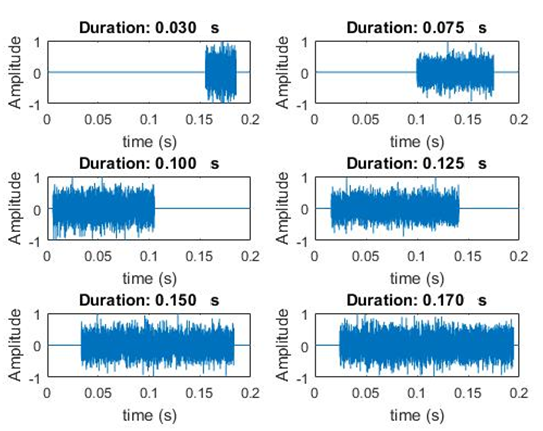
\includegraphics[width=\textwidth]{images/bursts.png}
  \caption{Σήματα λευκού θορύβου που χρησιμοποιήθηκαν ως είσοδος στο μοντέλο.}
  \label{fig:input_signals_examples}
\end{figure}



\section{Δημιουργία αμφιωτικών σημάτων} \label{sec:bin_sig_creation}

\noindent
Τα σήματα που περιγράφονται στην υποενότητα \ref{sec:input_signals} στη συνέχεια συνελίσονται με BRIRs, για διαφορετικές γωνίες, που προέρχονται από τρία δωμάτια: Το TU Berlin Auditorium 3 \cite{Wierstorf2016b}, το Spirit \cite{Wierstorf2016a}, και το Calypso \cite{Wierstorf2016}. Σε κάθε περίπτωση, το ανδρείκελο απείχε 1m από την πηγή, ενώ έγιναν μετρήσεις με ανάλυση $1^o$ στο οριζόντιο επίπεδο, από $-90^o$ μέχρι $+90^o$ χρησιμοποιώντας το ανδρείκελο KEMAR και ηχεία Genelec, τοποθετημένα σε ανύψωση $0^o$. 

Στην εργασία αυτή χρησιμοποιήθηκε ανάλυση στο οριζόντιο επίπεδο $2^o$, με αποτέλεσμα να προκύψουν 91 κρουστικές για κάθε δωμάτιο. Χρησιμοποιήθηκαν και τα τρία δωμάτια, και άρα μετά από τη συνέλιξη κάθε ενός από τα 29 σήματα εισόδου, με μία από τις $3 * 91 = 273$ διαφορετικές κρουστικές, δημιουργούνται συνολικά $29 * 273 = 7917$ διαφορετικά σήματα εισόδου.

Αναλυτικότερα, αφού φορτωθεί το εκάστοτε dataset, και από αυτό διαβαστεί η BRIR, η οποία εμφανώς αποτελείται από δύο κανάλια διότι είναι binaural, εφαρμόζεται σε αυτή ένα παράθυρο Half Hanning μήκους 9000 δειγμάτων, αφού ρυθμιστεί η ζητούμενη δειγματοληψία. Τα δύο κανάλια της BRIR συνελίσονται με το mono σήμα εισόδου και προκύπτει το αμφιωτικό σήμα από το οποίο θα εξαχθούν στη συνέχεια οι αμφιωτικές παράμετροι. Έτσι, το αποτέλεσμα της συνέλιξης είναι ένα αμφιωτικό σήμα διαστάσεων $[2,L]$, όπου $L = M + N - 1 = 17819$, με δεδομένο ότι η BRIR έχει μήκος $M = 9000$ δείγματα και το mono σήμα μήκος $N = 8820$ δείγματα.

Η παραθύρωση έγινε λόγω περιορισμών στους υπολογιστικούς πόρους, αλλά επιλέχθηκε τέτοιο μέγεθος παραθύρου ώστε να διατηρούνται τα σημαντικότερα χαρακτηριστικά των BRIR. 

Μια κρουστική μαζί με το παράθυρο που εφαρμόζεται σε αυτή και η BRIR μετά την εφαρμογή του, φαίνονται στο Σχήμα \ref{fig:brir_processing}. Συνοπτικά η διαδικασία της δημιουργίας των αμφιωτικών σημάτων φαίνεται στο Σχήμα \ref{fig:binaural_signal_gen_block}.

\begin{figure}[h]
  \centering
  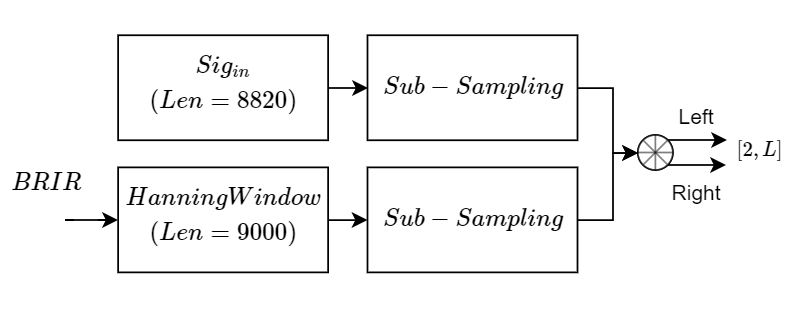
\includegraphics[width=\textwidth]{images/binaural_signal_gen_block.png}
  \caption{Δημιουργία αμφιωτικών σημάτων. Το block sub-sampling χρησιμοποιείται μόνο στην περίπτωση που τα σήματα έχουν διαφορετική δειγματοληψία από την επιθυμητή $f_s = 44.1 kHz$}
  \label{fig:binaural_signal_gen_block}
\end{figure}

\begin{figure}
     \centering
     \begin{subfigure}[b]{\textwidth}
         \centering
         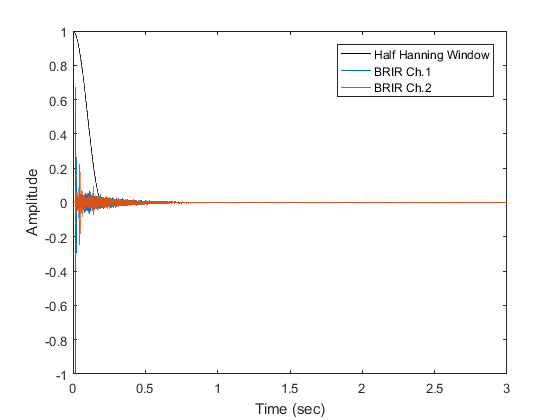
\includegraphics[width=\textwidth]{images/brir_window.png}
         \caption{}
         \label{fig:brir_window}
     \end{subfigure}
     \hfill
     \begin{subfigure}[b]{\textwidth}
         \centering
         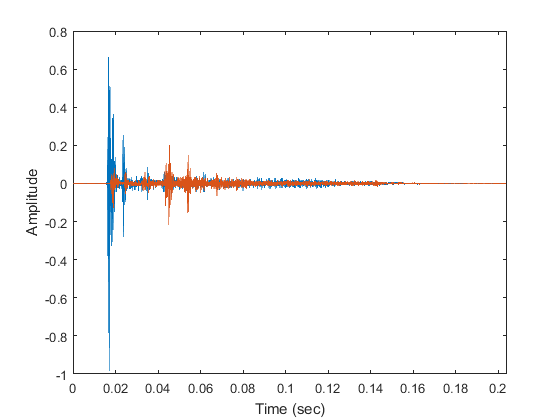
\includegraphics[width=\textwidth]{images/windowed_brir.png}
         \caption{}
         \label{fig:windowed_brir}
     \end{subfigure}
        \caption{(α'): BRIR και το αντίστοιχο Half Hanning παράθυρο, (β'): BRIR μετά την παραθύρωση. Τα σχήματα είναι για $f_s = 44.1 kHz$ }
        \label{fig:brir_processing}
\end{figure}

\section{Εξαγωγή αμφιωτικών παραμέτρων}

\noindent
Σε αυτή την ενότητα, αναλύεται η εφαρμογή του μοντέλου του Dietz το θεωρητικό υπόβαθρο του οποίου περιγράφεται στην υποενότητα \ref{sec:dietz_theory}. Η συνάρτηση είναι υλοποιημένη σε MATLAB, στο Auditory Modeling Toolbox. Η συνάρτηση χρειάζεται ως ορίσματα το binaural σήμα και τη συχνότητα δειγματοληψίας, ενώ στην έξοδό της δίνονται οι αμφιωτικές παράμετροι.

Συνοπτικά η διαδικασία που ακολουθείται για τον υπολογισμό των παραμέτρων, φαίνεται στο Σχήμα \ref{fig:dietz_block_diagram_MATLAB} και τα επιμέρους στοιχεία της αναλύονται στη συνέχεια.

\begin{figure}[h]
  \centering
  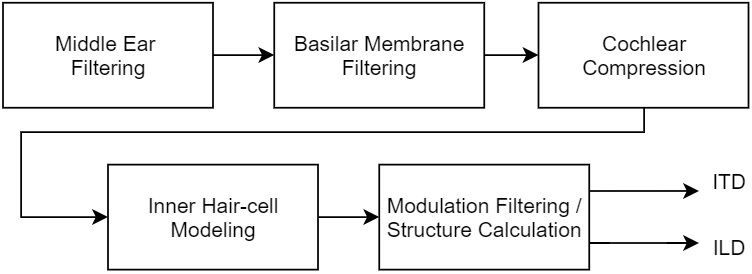
\includegraphics[width=\textwidth]{images/dietz_block_diagram_MATLAB.png}
  \caption{Συνοπτική περιγραφή της υλοποίησης του μοντέλου Dietz για το ακουστικό σύστημα.}
  \label{fig:dietz_block_diagram_MATLAB}
\end{figure}

\noindent
Αξίζει εδώ να σημειωθεί πως η υλοποίηση του μοντέλου, πιστώνεται στους:
\begin{itemize}
    \item Tobias Peters (tobias@medi.physik.uni-oldenburg.de)
    \item Mathias Dietz (mathias.dietz@uni-oldenburg.de)
    \item Martin Klein-Hennig (martin.klein.hennig@uni-oldenburg.de)
\end{itemize}{}

Παρακάτω, μελετάται η λειτουργία του μοντέλου, με βάση ένα  από τα binaural σήματα εισόδου που χρησιμοποιούνται, που αντιστοιχεί σε γωνία άφιξης $+80^o$ από το δωμάτιο Spirit, όπως φαίνεται στο Σχήμα \ref{fig:example_bin_sig}.

\begin{figure}[h]
  \centering
  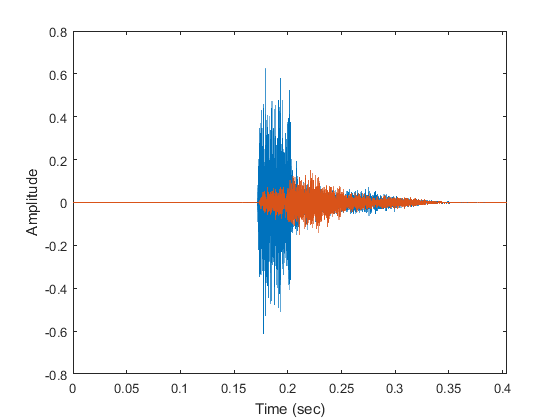
\includegraphics[width=\textwidth]{images/example_bin_sig.png}
  \caption{Binaural σήμα για γωνία άφιξης $+80^o$, στο δωμάτιο Spirit.}
  \label{fig:dietz_out}
\end{figure}

\subsection{Φιλτράρισμα Μέσου Αυτιού}

Αρχικά, το σήμα περνά από ένα bandpass butterworth φίλτρο με $f_{c1} = 500 Hz$ και $f_{c2} = 2 kHz$ το οποίο φαίνεται στο Σχήμα \ref{fig:butterworth_dietz_1}, ενώ το τελικό αποτέλεσμα της επεξεργασίας φαίνεται στο Σχήμα \ref{fig:dietz_out1}. Όπως είναι αναμενόμενο, όντας ουσιαστικά σήμα λευκού θορύβου, η μορφή του αλλάζει αισθητά στο πεδίο του χρόνου, αφού μειώνεται σημαντικά το υψίσυχνο περιεχόμενο.

\begin{figure}[h!]
  \centering
  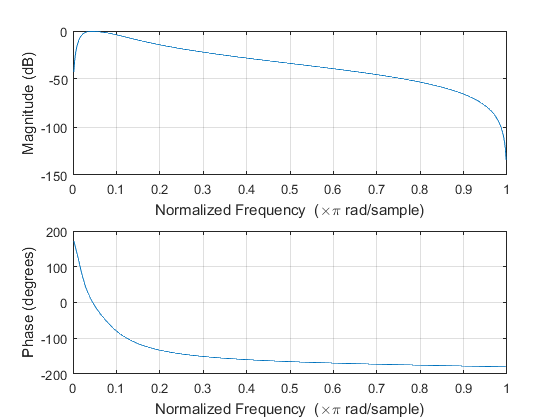
\includegraphics[width=\textwidth,height=8cm]{images/butterworth_dietz_1.png}
  \caption{IIR φίλτρο τύπου butterworth που προσομοιώνει το φιλτράρισμα του μέσου αυτιού.}
  \label{fig:butterworth_dietz_1}
\end{figure}

\begin{figure}[h!]
  \centering
  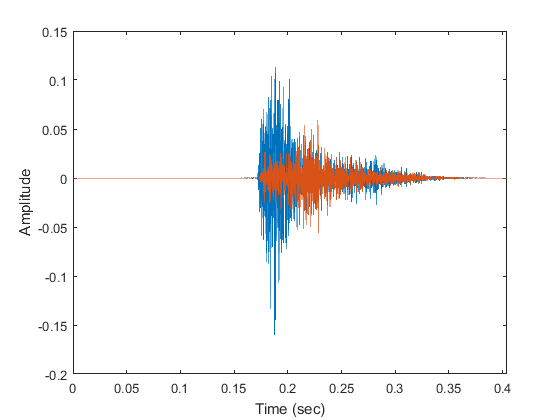
\includegraphics[width=\textwidth]{images/dietz_out1.png}
  \caption{Αποτέλεσμα της επεξεργασίας του μέσου αυτιού.}
  \label{fig:dietz_out1}
\end{figure}

\subsection{Προσομοίωση Εσωτερικού Αυτιού}

Σε αυτό το σημείο, για την προσομοίωση της basilar μεμβράνης, υπολογίζονται 23 gammatone φίλτρα με μιγαδικούς συντελεστές για τον υπολογισμό της ITF (Εξίσωση \ref{eq:ITF}). Το πλήθος των φίλτρων προκύπτει από το γεγονός ότι μεταξύ τους απέχουν 1 ERB, το οποίο αντιστοιχίζεται σε περίπου 217 Hz, και καλύπτουν το διάστημα 200 - 5000 Hz. Η κρουστική απόκριση ενός gammatone φίλτρου, περιγράφεται στην Εξίσωση \ref{eq:gammatone_IR}. Ουσιαστικά είναι ένα φίλτρο που προκύπτει από τον πολλαπλασιασμό μιας κατανομής γάμμα, και ενός ημιτονοειδούς τόνου. Οι αποκρίσεις συχνότητας των 23 φίλτρων παρουσιάζονται στο Σχήμα \ref{fig:gammatone_responses}. Το αποτέλεσμα του φιλτραρίσματος, είναι μιγαδικό, και αποτελείται από 23 συχνοτικές μπάντες.

\begin{CEquation}
    g(t) = \alpha t^{n-1}\cos{(2\pi f_c t)}e^{-2\pi\beta t}
    \label{eq:gammatone_IR}
\end{CEquation}

\begin{figure}[h]
  \centering
  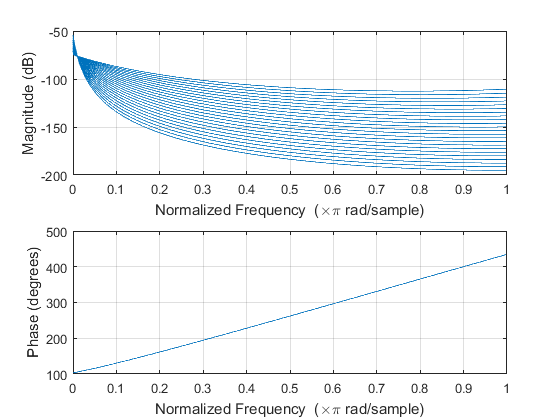
\includegraphics[width=\textwidth]{images/gammatone_responses.png}
  \caption{Αποκρίσεις συχνότητας της τράπεζας φίλτρων gammatone.}
  \label{fig:gammatone_responses}
\end{figure}

Στη συνέχεια για τη μοντελοποίηση της συμπίεσης του κοχλία χρησιμοποιείται η Εξίσωση \ref{eq:cochlear_compression} δείγμα προς δείγμα. Ακολούθως, τα εσωτερικά hair-cells του αυτιού μοντελοποιούνται όπως έχει ήδη αναφερθεί με μια ανόρθωση ημίσεος κύματος και στη συνέχεια ένα lowpass φίλτρο, με αποτέλεσμα την εξαγωγή μια 'περιβάλλουσας'. Στο σημείο αυτό, το ένα εκ των δύο καναλιών του σήματος, έχει τη μορφή που φαίνεται στο Σχήμα \ref{fig:dietz_out2}.

\begin{CEquation}
    y(n) = sign(x(n)) * |x(n)| ^ c
    \label{eq:cochlear_compression}
\end{CEquation}

\begin{figure}[h]
  \centering
  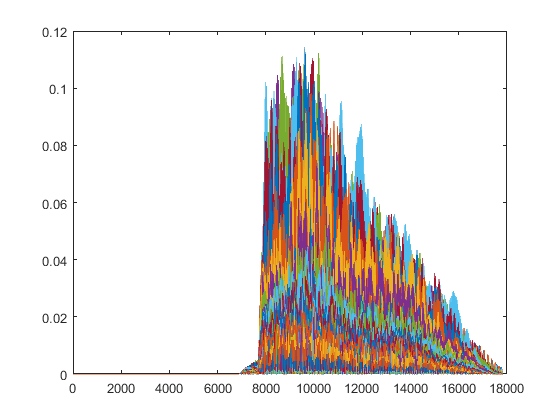
\includegraphics[width=\textwidth]{images/dietz_out2.png}
  \caption{Έξοδος του μοντέλου μετά τη μοντελοποίηση του εσωτερικού αυτιού.}
  \label{fig:dietz_out2}
\end{figure}

\subsection{Τράπεζα Φίλτρων Διαμόρφωσης}

Το επόμενο στάδιο της επεξεργασίας περιέχει ακόμα μια τράπεζα φίλτρων, που αποτελείται από τρία gammatone φίλτρα 2ης τάξης, για τον διαχωρισμό στις δομές 'fine' και 'envelope' που περιέχουν πληροφορία χαμηλών (κάτω από 1.4 kHz) και υψηλών συχνοτήτων αντίστοιχα και ένα lowpass με $f_c = 30 Hz$ για τον υπολογισμό του ILD. Κατ' επέκταση, η fine δομή έχει 12 διαστάσεις, που κάθε μια αντιστοιχεί σε συχνοτικές μπάντες από $200-1400 Hz$ ενώ η δομή envelope 11 διαστάσεις που αντιστοιχούν στις εναπομείνασες συχνότητες. Τα προαναφερθέντα φίλτρα, εφαρμόζονται σε κάθε μία από τις συχνοτικές μπάντες της εξόδου του προηγούμενου σταδίου. Οι έξοδοι σε αυτό το σημείο, λόγω των μιγαδικών συντελεστών των gammatone φίλτρων είναι πάλι μιγαδικές.

\subsection{Αμφιωτικός επεξεργαστής}

Το τελευταίο στάδιο της επεξεργασίας, υλοποιείται από τον binaural processor, o οποίος εφαρμόζει τις εξισώσεις που έχουν περιγραφεί αναλυτικά στο κεφάλαιο \ref{sec:dietz_theory} στις δομές fine και envelope. Τα τελικά αποτελέσματα, για τις αμφιωτικές παραμέτρους που αφορούν αυτή την εργασία, παρουσιάζονται στο Σχήμα \ref{fig:dietz_out_final}.

\begin{figure}[h]
  \centering
  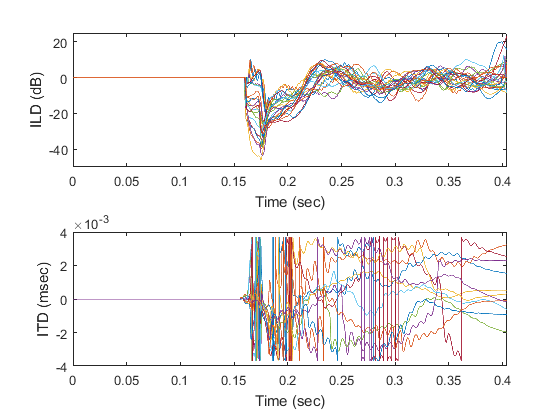
\includegraphics[width=\textwidth]{images/dietz_out_final.png}
  \caption{Τελικές έξοδοι του μοντέλου: (Πάνω) ILD για 23 συχνοτικές μπάντες, (Κάτω) ITD για την δομή envelope - 11 μπάντες.}
  \label{fig:dietz_out_final}
\end{figure}


\section{Συμπίεση Δεδομένων} \label{sec:data_compression}
\noindent
Σε αυτή την ενότητα, αναλύονται τα βήματα που ακολουθήθηκαν για την μείωση των δεδομένων των αμφιωτικών παραμέτρων, καθώς και τα κίνητρα πίσω από αυτή. Έγινε προσπάθεια για την επίτευξη της μέγιστης ευελιξίας, λόγω των δεδομένων, ως προς τις δομές των ΝΝ που μπορούσαν να χρησιμοποιηθούν, αφού μεγάλα παραδείγματα εισόδου, εισάγουν περιορισμούς ως προς το πλήθος των κρυφών επιπέδων που μπορούν να χρησιμοποιηθούν, αλλά και το πλήθος των νευρώνων σε κάθε ένα από αυτά. Η συμπίεση συμβαίνει σε δύο στάδια. Στο πρώτο, τα δεδομένα συμπιέζονται με βάση με βάση ψυχοακουστικά μοντέλα ως προς την αντίληψη του ήχου, που υποδεικνύουν τις σημαντικές μπάντες κάθε παραμέτρου, ενώ στο δεύτερο εφαρμόζεται ο αλγόριθμος συμπίεσης που σχεδιάστηκε, για την εξαγωγή των 'προφίλ' των παραμέτρων. Συνοπτικά η συμπίεση περιγράφεται στο Σχήμα \ref{fig:Compression_block_diagram}, όπου με $P$ σημειώνεται η παράμετρος ενδιαφέροντος, $N_{dim}$ οι αρχικές διαστάσεις της, και με $N'_{dim}$ οι μειωμένες διαστάσεις. Τα στοιχεία του διαγράμματος αναλύονται περαιτέρω στις επόμενες υποενότητες.

\begin{figure}[h]
  \centering
  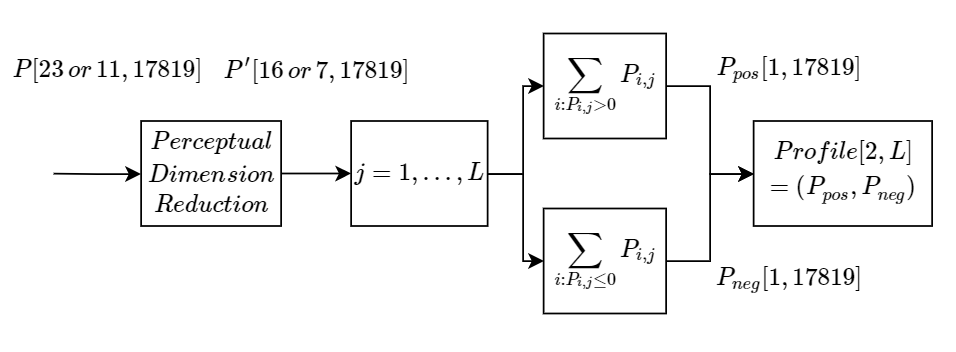
\includegraphics[width=\textwidth]{images/Compression_block_diagram.png}
  \caption{Προτεινόμενη μέθοδος συμπίεσης για τις αμφιωτικές παραμέτρους.}
  \label{fig:Compression_block_diagram}
\end{figure}

\subsection{Κίνητρο}

Για να γίνει σαφές το σκεπτικό πίσω από την επιλογή για τη συμπίεση των δεδομένων, είναι απαραίτητο να γίνει σαφές το μέγεθος των δεδομένων που το ακουστικό μοντέλο δίνει ως έξοδο. Όπως έχει αναφερθεί, το ILD έχει σε αυτό το σημείο 23 διαστάσεις και το ITD 11, κάθε μία από τις οποίες αντιστοιχεί σε μια μπάντα συχνοτήτων. Κάθε διάσταση έχει τον ίδιο αριθμό δειγμάτων με όλες τις υπόλοιπες, οπότε μπορούμε να πούμε ότι έχουμε συνολικά $23 + 11 = 34$ διαστάσεις δεδομένων. Το ακουστικό μοντέλο εκτελεί τις πράξεις της συνέλιξης, χωρίς να αυξάνει το πλήθος των δειγμάτων, οπότε κάθε διάσταση, όπως έχει αναφερθεί στην ενότητα \ref{sec:bin_sig_creation}, έχει $17819$, σημεία. Συνεπώς, προκύπτουν $34 * 17819 = 605846$ δείγματα. Γίνεται αμέσως αντιληπτό, πως το πλήθος των δειγμάτων, καθιστά το διάνυσμα απαγορευτικό για χρήση στην εκπαίδευση ενός νευρωνικού δικτύου, τόσο από άποψη του χρόνου που θα απαιτούνταν για την εκπαίδευση ενός τέτοιου μοντέλου, όσο και από την άποψη των περιορισμένων υπολογιστικών πόρων που είναι διαθέσιμοι.

\subsection{Αντιληπτική Συμπίεση}

Όπως έχει αναφερθεί στην ενότητα \ref{sec:binaural_cues}, αναλόγως με τη συχνότητα, η κάθε παράμετρος αποκτά διαφορετική βαρύτητα στον εντοπισμό ακουστικών πηγών. Με το ILD, να παίζει μεγαλύτερο ρόλο στις συχνότητες που είναι μεγαλύτερες από $1500 Hz$, ενώ το ITD το αντίθετο. Με βάση τις εξόδους του μοντέλου, και τη γνώση ότι κάθε μία από τις διαστάσεις των παραμέτρων αντιστοιχεί σε πλάτος 1 ERB, είναι αρκετά εύκολο να γίνει η αντιστοίχηση διαστάσεων-συχνοτικών μπαντών. Σε αυτή την εργασία, το crossover frequency, αντί για $1500 Hz$ τέθηκε κοντά στα $2000 Hz$, ώστε να υπάρχει μεγαλύτερη ισορροπία στο πλήθος των σημείων του ITD και του ILD. Σημειώνεται και εδώ πως χρησιμοποιείται η envelope δομή του μοντέλου.
Πιο συγκεκριμένα, από το ILD διατηρούνται οι διαστάσεις $8-23$, ενώ από το ITD οι $1-7$, όπως φαίνεται στην Εξίσωση \ref{eq:compression_1}. Τα αποτελέσματα της αντιληπτικής συμπίεσης παρουσιάζονται στα Σχήματα \ref{fig:ILD_Perceptual_Comp} και \ref{fig:ITD_Perceptual_Comp}.

\begin{CEquation}
\begin{split}
    ILD_{new} = ILD[8:23,:]\\
    ITD_{new} = ITD[1:7,:]
    \label{eq:compression_1}
\end{split}
\end{CEquation}

\begin{figure}[h]
  \centering
  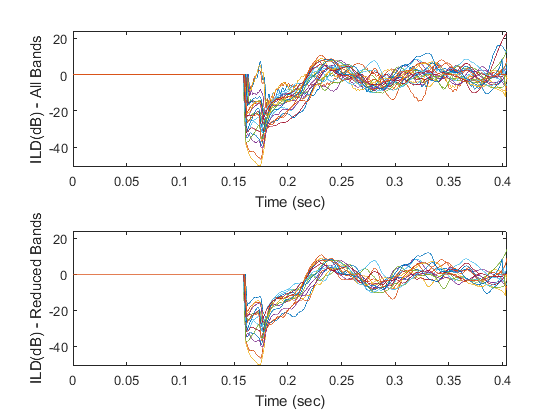
\includegraphics[width=\textwidth]{images/ILD_Perceptual_Comp.png}
  \caption{Σύγκριση πριν και μετά τη συμπίεση, της παραμέτρου ILD.}
  \label{fig:ILD_Perceptual_Comp}
\end{figure}

\begin{figure}[h]
  \centering
  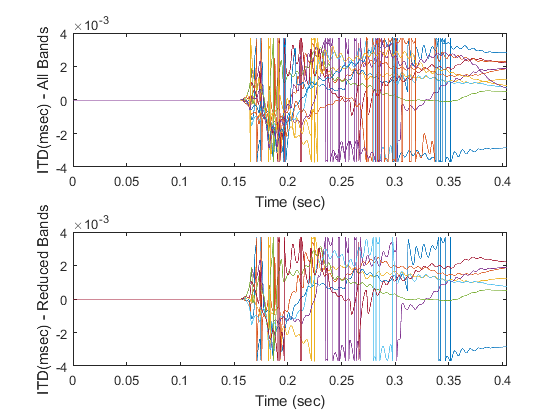
\includegraphics[width=\textwidth]{images/ITD_Perceptual_Comp.png}
  \caption{Σύγκριση πριν και μετά τη συμπίεση, της παραμέτρου ITD.}
  \label{fig:ITD_Perceptual_Comp}
\end{figure}

\sectionbreak
\subsection{Αλγοριθμική Συμπίεση}
Από τις παραμέτρους που προκύπτουν από την αντιληπτική συμπίεση, ο στόχος είναι ο υπολογισμός δύο χαρακτηριστικών καμπυλών, 'προφίλ', με σημαντικά μειωμένο μέγεθος δεδομένων, μία για τις θετικές και μία για τις αρνητικές τιμές κάθε παραμέτρου. Ο αλγόριθμος προσπελαύνει τις παραμέτρους ως προς το $L$, δηλαδή τη 'μεγάλη' διάσταση, και υπολογίζει δύο διαφορετικά αθροίσματα, ένα για τις θετικές τιμές κάθε διάστασης και ένα για τις αρνητικές, για το δείγμα $i$, και διαιρεί κάθε ένα από τα αθροίσματα με το πλήθος των στοιχείων που ανατέθηκαν σε αυτό, όπως φαίνεται στις Εξισώσεις \ref{eq:positive_profile} και \ref{eq:negative_profile}. Στη συνέχεια, τα δύο διανύσματα, συνδυάζονται στο τελικό προφίλ της παραμέτρου $Profile[2,L]$, όπως φαίνεται στην Εξίσωση \ref{eq:final_profile}. Τυπικά αποτελέσματα του αλγορίθμου φαίνονται στο Σχήμα \ref{fig:profiles_example}. Ο αλγόριθμος είναι απλός στην υλοποίηση και γρήγορος στην εκτέλεση, οπότε ενδείκνυται για την επεξεργασία ιδιαίτερα μεγάλων dataset. Ο λόγος συμπίεσης του αλγορίθμου δίνεται στην Εξίσωση \ref{eq:compression_ratio} και στη συγκεκριμένη εφαρμογή είναι $CR = 88.24\%$. Τα αποτελέσματα των μοντέλων που εκπαιδεύτηκαν με τα δεδομένα που έχουν επεξεργαστεί από τον προτεινόμενο αλγόριθμο είναι με διαφορά καλύτερα σε σχέση με άλλες μεθόδους επεξεργασίας και θεωρείται πως αυτό συμβαίνει διότι διατηρούνται τα σημαντικότερα χαρακτηριστικά των αμφιωτικών σημάτων, που πιστεύεται πως είναι οι κορυφές που προκύπτουν στο onset / offset του burst.

\begin{CEquation}
\begin{split}
    P_{pos} = \frac{\sum_{i:P_{i,j}>0}P_{i,j}}{\sum_{i:P_{i,j}>0}1}
    \label{eq:positive_profile}
\end{split}
\end{CEquation}

\begin{CEquation}
\begin{split}
    P_{neg} = \frac{\sum_{i:P_{i,j}<0}P_{i,j}}{\sum_{i:P_{i,j}<0}1}
    \label{eq:negative_profile}
\end{split}
\end{CEquation}

\begin{CEquation}
\begin{split}
    Profile[2,L] = (P_{pos}, P_{neg})
    \label{eq:final_profile}
\end{split}
\end{CEquation}

\begin{figure}[h]
  \centering
  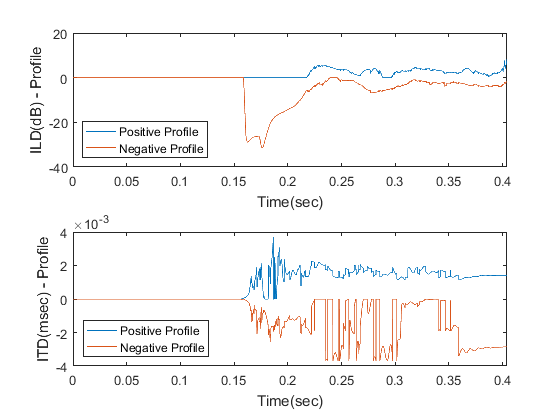
\includegraphics[width=\textwidth]{images/profiles_example.png}
  \caption{Προφίλ αμφιωτικών παραμέτρων: (Πάνω): ILD, (Κάτω): ITD.}
  \label{fig:profiles_example}
\end{figure}

\begin{CEquation}
\begin{split}
    CR = \frac{4*L}{N'_{dim}*L} = \frac{4}{N'_{dim}}
    \label{eq:compression_ratio}
\end{split}
\end{CEquation}

\section{Προεπεξεργασία Δεδομένων}
\noindent
Το επόμενο στάδιο του συστήματος εκτίμησης DOA, είναι η προεπεξεργασία των συμπιεσμένων αμφιωτικών παραμέτρων, ώστε να μπορούν να χρησιμοποιηθούν για την εκπαίδευση ενός ΝΝ. Στη μηχανική μάθηση, η διαδικασία της προεπεξεργασίας, εκτιμάται ότι είναι τόσο σημαντική όσο και η διαδικασία της κατασκευής του μοντέλου. Παρόλα αυτά όμως, λόγω της πρόσφατης άνθησης του τομέα της μηχανικής μάθησης, δεν υπάρχει αρκετή εμπειρία πάνω σε αυτόν και κατ' επέκταση δεν είναι γνωστός ο καλύτερος τρόπος προεπεξεργασίας των δεδομένων, ανάλογα με τον τύπο τους. Αν και υπάρχουν μερικές τεχνικές οι οποίες είναι ευρέως αποδεκτό ότι παρέχουν καλά αποτελέσματα, επί το πλείστον, οι ερευνητές προσεγγίζουν το πρόβλημα μέσω trial and error.

Μια από τις ευρέως γνωστές τεχνικές προεπεξεργασίας δεδομένων, είναι αυτή της κανονικοποίησης των τιμών των παραμέτρων, ώστε να αποφευχθεί ο κορεσμός του δικτύου όταν προκύπτουν πολύ μεγάλα βάρη στις συνάψεις. Με αυτόν τον τρόπο επιταχύνεται επίσης η διαδικασία της εκπαίδευσης του μοντέλου \cite{Sola1997,Lecun2012}. Εδώ η κανονικοποίηση, έγινε στο κλειστό διάστημα $[-1,1]$, και κρίθηκε πως είναι απαραίτητη λόγω της μεγάλης διαφοράς τάξεως μεγέθους μεταξύ των τιμών της παραμέτρου ILD, η οποία μετριέται σε dB, και της παραμέτρου ITD, η οποία μετριέται σε msec. Με αυτόν τον τρόπο υποδεικνύεται στο μοντέλο, ότι οι παράμετροι πρέπει να αντιμετωπιστούν με την ίδια βαρύτητα. 

Τα προφίλ των παραμέτρων, με διαστάσεις $[2,L]$, μετασχηματίζονται σε διανύσματα γραμμής, με διαστάσεις $[1,2L]$, όπως φαίνεται στην Εξίσωση \ref{eq:profile_flattening}. Τα δύο διανύσματα γραμμής διαστάσεων $[1,2L]$, τελικά συνδυάζονται στο διάνυσμα που θα αποτελέσει την είσοδο του νευρωνικού, με ένα τυπικό παράδειγμα να φαίνεται στο Σχήμα \ref{fig:final_profile}. Σημειώνεται πως τα δεδομένα μετά την προεπεξεργασία χάνουν τη φυσική σημασία τους. 
\begin{CEquation}
\begin{split}
    Input\;Vector[1:L] = Profile[1,L]\\
    Input\;Vector[L+1:2L] = Profile[2,L]
    \label{eq:profile_flattening}
\end{split}
\end{CEquation}
Από τα 7917 διαφορετικά διανύσματα που υπολογίζονται, το 80\% χρησιμοποιείται για την εκπαίδευση του νευρωνικού, το 10\% χρησιμοποιείται για validation, και το υπόλοιπο 10\% για testing. Κάθε διάνυσμα είναι μοναδικό, και αντιστοιχεί σε μία μετάθεση DOA-σήματος εισόδου-δωματίου. Η διαδικασία του διαχωρισμού σε train-validation-test data γίνεται με τυχαίο τρόπο, ώστε τα αποτελέσματα να είναι αξιόπιστα και γενικεύσιμα.

\begin{figure}[h]
  \centering
  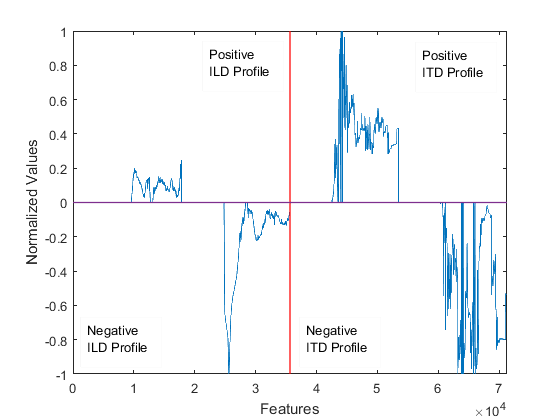
\includegraphics[width=\textwidth]{images/final_profile.png}
  \caption{Τυπικό παράδειγμα κανονικοποιημένου διανύσματος εισόδου στο ΝΝ από τις αμφιωτικές παραμέτρους για συγκεκριμένη γωνία άφιξης.}
  \label{fig:final_profile}
\end{figure}

\section{Αρχιτεκτονικές Νευρωνικών Δικτύων}
\noindent

Ο όρος \textit{'αρχιτεκτονική ANN'} αναφέρεται στην διάταξη των νευρώνων σε επίπεδα, τις συνδέσεις μεταξύ των επιπέδων, τις συναρτήσεις ενεργοποίησης και τις μεθόδους μάθησης \cite{Kalogirou_2014}. Απλούστερα, γίνεται σαφές ότι αναφέρεται στο σύνολο της κατασκευής ενός NN. Το \textit{μοντέλο} του ΝΝ, και η αρχιτεκτονική του, καθορίζουν τον τρόπο που η είσοδος παράγει με υπολογιστικό τρόπο μια έξοδο. Η βασική λειτουργία που πρέπει να ακολουθηθεί για την σωστή αντιμετώπιση ενός προβλήματος, είναι όπως φαίνεται, αυτή της επιλογής της σωστής αρχιτεκτονικής καθώς και των υπερπαραμέτρων που αναλύονται στην υποενότητα \ref{subsub:hyperparameters}. Εξίσου σημαντική, είναι η επιλογή της αντικειμενικής συνάρτησης, η οποία συχνά αποκαλείται και συνάρτηση απώλειας (loss function), που είναι επιθυμητό να ελαχιστοποιηθεί (ή να μεγιστοποιηθεί αναλόγως με το πρόβλημα). Σε αυτή την εργασία, τα μοντέλα προσπαθούν να ελαχιστοποιήσουν το \textit{Μέσο Τετραγωνικό Σφάλμα} (MSE), ενώ κατά την εκπαίδευσή τους παρακολουθείται το Μέσο Απόλυτο Σφάλμα (MAE) και η Ρίζα του Μέσου Τετραγωνικού Σφάλματος (RMSE). Δοκιμάστηκε η απόδοση αρκετών διαφορετικών μοντέλων, εδώ όμως αναλύονται τα καλύτερα εκ των δύο ευρύτερων κατηγοριών, των πλήρως διασυνδεδεμένων (Fully Connected), και των συνελικτικών (Convolutional). Εδώ σημειώνεται πως η προεπεξεργασία των δεδομένων, καθώς και τα ίδια τα μοντέλα έχουν υλοποιηθεί με τη βοήθεια της βιβλιοθήκης TensorFlow στη γλώσσα Python. Στο πακέτο αυτό προστέθηκαν μερικές custom συναρτήσεις για την λεπτομερέστερη παρακολούθηση του χρόνου εκτέλεσης.

\subsection{Fully Connected}
Το πλήρως διασυνδεδεμένο μοντέλο που έδωσε τα καλύτερα αποτελέσματα, απεικονίζεται στο Σχήμα \ref{fig:FC_Arch}, και αποτελείται από ένα επίπεδο εισόδου με 71276 νευρώνες, τέσσερα κρυφά επίπεδα με 2000, 360, 180 και 90 νευρώνες αντίστοιχα, καθώς και το επίπεδο εξόδου, που έχει έναν νευρώνα που δίνει την πρόβλεψη. Μετά το επίπεδο εισόδου, καθώς και μετά από το 1ο κρυφό επίπεδο, τοποθετείται ένα επίπεδο Dropout, το οποίο δεν αποτελείται από νευρώνες, αλλά ελέγχει τους νευρώνες του προηγούμενου επιπέδου. Όλα τα επίπεδα που περιέχουν νευρώνες, χρησιμοποιούν την ReLU (εξίσωση \ref{eq:ReLU}) ως συνάρτηση ενεργοποίησης.

Αναλυτικότερα, η εκπαίδευση έγινε χρησιμοποιώντας, όπως έχει ήδη αναφερθεί, ως συνάρτηση απώλειας το MSE, και τον βελτιστοποιητή Adam (Adaptive Moment Estimation) με αρχικό ρυθμό μάθησης $Lr = 0.001$. 

\begin{figure}[h]
\centering
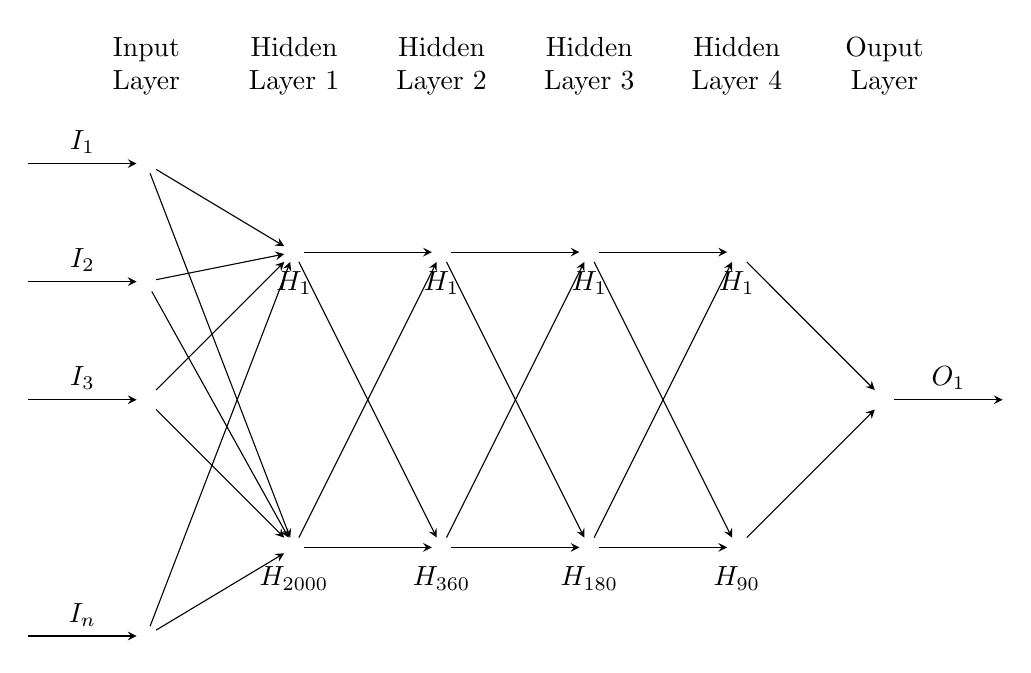
\begin{tikzpicture}[x=1.5cm, y=1.5cm, >=stealth]

\foreach \m/\l [count=\y] in {1,2,3,missing,4}
  \node [every neuron/.try, neuron \m/.try] (input-\m) at (0,2.5-\y) {};

\foreach \m [count=\y] in {1,missing,2}
  \node [every neuron/.try, neuron \m/.try ] (1-hidden-\m) at (1.25,2-\y*1.25) {};

\foreach \m [count=\y] in {1,missing,2}
  \node [every neuron/.try, neuron \m/.try ] (2-hidden-\m) at (2.5,2-\y*1.25) {};
  
 \foreach \m [count=\y] in {1,missing,2}
  \node [every neuron/.try, neuron \m/.try ] (3-hidden-\m) at (3.75,2-\y*1.25) {};

\foreach \m [count=\y] in {1,missing,2}
  \node [every neuron/.try, neuron \m/.try ] (4-hidden-\m) at (5,2-\y*1.25) {};
  
  
\foreach \m [count=\y] in {1}
  \node [every neuron/.try, neuron \m/.try ] (output-\m) at (6.25,\y-1.5) {};

\foreach \l [count=\i] in {1,2,3,n}
  \draw [<-] (input-\i) -- ++(-1,0)
    node [above, midway] {$I_\l$};

\foreach \l [count=\i] in {1,2000}
  \node [below] at (1-hidden-\i.south) {$H_{\l}$};
  
  \foreach \l [count=\i] in {1,360}
  \node [below] at (2-hidden-\i.south) {$H_{\l}$};

\foreach \l [count=\i] in {1,180}
  \node [below] at (3-hidden-\i.south) {$H_{\l}$};

\foreach \l [count=\i] in {1,90}
  \node [below] at (4-hidden-\i.south) {$H_{\l}$};
  
  
\foreach \l [count=\i] in {1}
  \draw [->] (output-\i) -- ++(1,0)
    node [above, midway] {$O_\l$};

\foreach \i in {1,...,4}
  \foreach \j in {1,...,2}
    \draw [->] (input-\i) -- (1-hidden-\j);

\foreach \i in {1,...,2}
  \foreach \j in {1,...,2}
    \draw [->] (1-hidden-\i) -- (2-hidden-\j);

\foreach \i in {1,...,2}
  \foreach \j in {1,...,2}
    \draw [->] (2-hidden-\i) -- (3-hidden-\j);

\foreach \i in {1,...,2}
  \foreach \j in {1,...,2}
    \draw [->] (3-hidden-\i) -- (4-hidden-\j);

    
\foreach \i in {1,...,2}
  \foreach \j in {1}
    \draw [->] (4-hidden-\i) -- (output-\j);

\foreach \l [count=\x from 0] in {Input\\Layer, Hidden\\Layer 1, Hidden\\Layer 2, Hidden\\Layer 3, Hidden\\Layer 4, Ouput\\Layer}
  \node [align=center, above] at (\x*1.25,2) {\l};

\end{tikzpicture}
\caption{Fully connected χωρίς τα επίπεδα Dropout.}
\label{fig:FC_Arch}
\end{figure}

\subsubsection{Επίπεδο Dropout}
Με απλά λόγια, η λειτουργία του επιπέδου Dropout, είναι η απενεργοποίηση, με τυχαίο τρόπο, νευρώνων του προγηούμενου επιπέδου. Το επίπεδο αυτό, έχει μία υπερπαράμετρο, το \textit{Dropout Rate} (DR), το οποίο καθορίζει το πλήθος των νευρώνων που απενεργοποιούνται σε κάθε εποχή (ένα πέρασμα ολόκληρου του dataset από το νευρωνικό). Για παράδειγμα, για $DR=0.4$, με το προηγούμενο επίπεδο να έχει 2000 νευρώνες, σε κάθε εποχή απενεργοποιούνται οι $2000*0.4 = 800$ από αυτούς. Το αποτέλεσμα αυτής της διαδικασίας, είναι το νευρωνικό να μην βασίζεται αποκλειστικά σε μερικούς νευρώνες εκ του συνόλου για την τελική εκτίμηση που δίνει στην έξοδο μειώνοντας με αυτόν τον τρόπο σημαντικά το overfitting. Μια συνοπτική περιγραφή της λειτουργίας του επιπέδου, φαίνεται στο Σχήμα \ref{fig:dropout_ex}. Σε αυτό το σχήμα θεωρείται πως υπάρχει ένα Dropout Layer ενδιάμεσα από όλα τα επίπεδα.

\begin{figure}
\centering
\scalebox{.8}{
\hbox{\hspace{-2em}
\begin{tikzpicture}

	\node[circle, draw, thick] (i1) {};
	\node[circle, draw, thick, above=2em of i1] (i2) {};
	\node[circle, draw, thick, above=2em of i2] (i3) {};
	\node[circle, draw, thick, below=2em of i1] (i4) {};
	\node[circle, draw, thick, below=2em of i4] (i5) {};
	
	\node[circle, draw, thick, right=4em of i1] (h1) {};
	\node[circle, draw, thick, right=4em of i2] (h2) {};
	\node[circle, draw, thick, right=4em of i3] (h3) {};
	\node[circle, draw, thick, right=4em of i4] (h4) {};
	\node[circle, draw, thick, right=4em of i5] (h5) {};
	
	\node[circle, draw, thick, right=4em of h1] (hh1) {};
	\node[circle, draw, thick, right=4em of h2] (hh2) {};
	\node[circle, draw, thick, right=4em of h3] (hh3) {};
	\node[circle, draw, thick, right=4em of h4] (hh4) {};
	\node[circle, draw, thick, right=4em of h5] (hh5) {};
	
	\node[circle, draw, thick, right=4em of hh2] (o1) {};
	\node[circle, draw, thick, right=4em of hh4] (o2) {};
	
	\draw[-stealth, thick] (i1) -- (h1);
	\draw[-stealth, thick] (i1) -- (h2);
	\draw[-stealth, thick] (i1) -- (h3);
	\draw[-stealth, thick] (i1) -- (h4);
	\draw[-stealth, thick] (i1) -- (h5);
	\draw[-stealth, thick] (i2) -- (h1);
	\draw[-stealth, thick] (i2) -- (h2);
	\draw[-stealth, thick] (i2) -- (h3);
	\draw[-stealth, thick] (i2) -- (h4);
	\draw[-stealth, thick] (i2) -- (h5);
	\draw[-stealth, thick] (i3) -- (h1);
	\draw[-stealth, thick] (i3) -- (h2);
	\draw[-stealth, thick] (i3) -- (h3);
	\draw[-stealth, thick] (i3) -- (h4);
	\draw[-stealth, thick] (i3) -- (h5);
	\draw[-stealth, thick] (i4) -- (h1);
	\draw[-stealth, thick] (i4) -- (h2);
	\draw[-stealth, thick] (i4) -- (h3);
	\draw[-stealth, thick] (i4) -- (h4);
	\draw[-stealth, thick] (i4) -- (h5);
	\draw[-stealth, thick] (i5) -- (h1);
	\draw[-stealth, thick] (i5) -- (h2);
	\draw[-stealth, thick] (i5) -- (h3);
	\draw[-stealth, thick] (i5) -- (h4);
	\draw[-stealth, thick] (i5) -- (h5);
	
	\draw[-stealth, thick] (h1) -- (hh1);
	\draw[-stealth, thick] (h1) -- (hh2);
	\draw[-stealth, thick] (h1) -- (hh3);
	\draw[-stealth, thick] (h1) -- (hh4);
	\draw[-stealth, thick] (h1) -- (hh5);
	\draw[-stealth, thick] (h2) -- (hh1);
	\draw[-stealth, thick] (h2) -- (hh2);
	\draw[-stealth, thick] (h2) -- (hh3);
	\draw[-stealth, thick] (h2) -- (hh4);
	\draw[-stealth, thick] (h2) -- (hh5);
	\draw[-stealth, thick] (h3) -- (hh1);
	\draw[-stealth, thick] (h3) -- (hh2);
	\draw[-stealth, thick] (h3) -- (hh3);
	\draw[-stealth, thick] (h3) -- (hh4);
	\draw[-stealth, thick] (h3) -- (hh5);
	\draw[-stealth, thick] (h4) -- (hh1);
	\draw[-stealth, thick] (h4) -- (hh2);
	\draw[-stealth, thick] (h4) -- (hh3);
	\draw[-stealth, thick] (h4) -- (hh4);
	\draw[-stealth, thick] (h4) -- (hh5);
	\draw[-stealth, thick] (h5) -- (hh1);
	\draw[-stealth, thick] (h5) -- (hh2);
	\draw[-stealth, thick] (h5) -- (hh3);
	\draw[-stealth, thick] (h5) -- (hh4);
	\draw[-stealth, thick] (h5) -- (hh5);
	
	
	\draw[-stealth, thick] (hh1) -- (o1);
	\draw[-stealth, thick] (hh1) -- (o2);
	\draw[-stealth, thick] (hh2) -- (o1);
	\draw[-stealth, thick] (hh2) -- (o2);
	\draw[-stealth, thick] (hh3) -- (o1);
	\draw[-stealth, thick] (hh3) -- (o2);
	\draw[-stealth, thick] (hh4) -- (o1);
	\draw[-stealth, thick] (hh4) -- (o2);
	\draw[-stealth, thick] (hh5) -- (o1);
	\draw[-stealth, thick] (hh5) -- (o2);
	
	\draw[-stealth, double, dashed, thick] (5.5,0) -- node[above] {dropout} (8.6, 0);
	
	
	%%% BOUNDARY %%%
	
	\node[circle, draw, thick, red, fill=red!10, right=15em of hh1] (i1) {};
	\node[circle, draw, thick, red, fill=red!10, above=2em of i1] (i2) {};
	\node[circle, draw, thick, above=2em of i2] (i3) {};
	\node[circle, draw, thick, below=2em of i1] (i4) {};
	\node[circle, draw, thick, below=2em of i4] (i5) {};
	
	\node[red] (icr) at (i1) {$\mathlarger{\mathlarger{\mathlarger{\mathlarger{\mathlarger{\bm{\times}}}}}}$};
	\node[red] (icr) at (i2) {$\mathlarger{\mathlarger{\mathlarger{\mathlarger{\mathlarger{\bm{\times}}}}}}$};
	
	\node[circle, draw, thick, red, fill=red!10, right=4em of i1] (h1) {};
	\node[circle, draw, thick, right=4em of i2] (h2) {};
	\node[circle, draw, thick, red, fill=red!10, right=4em of i3] (h3) {};
	\node[circle, draw, thick, red, fill=red!10, right=4em of i4] (h4) {};
	\node[circle, draw, thick, right=4em of i5] (h5) {};
	
	\node[red] (icr) at (h1) {$\mathlarger{\mathlarger{\mathlarger{\mathlarger{\mathlarger{\bm{\times}}}}}}$};
	\node[red] (icr) at (h3) {$\mathlarger{\mathlarger{\mathlarger{\mathlarger{\mathlarger{\bm{\times}}}}}}$};
	\node[red] (icr) at (h4) {$\mathlarger{\mathlarger{\mathlarger{\mathlarger{\mathlarger{\bm{\times}}}}}}$};
	
	\node[circle, draw, thick, right=4em of h1] (hh1) {};
	\node[circle, draw, thick, red, fill=red!10, right=4em of h2] (hh2) {};
	\node[circle, draw, thick, right=4em of h3] (hh3) {};
	\node[circle, draw, thick, red, fill=red!10, right=4em of h4] (hh4) {};
	\node[circle, draw, thick, right=4em of h5] (hh5) {};
	
	\node[red] (icr) at (hh2) {$\mathlarger{\mathlarger{\mathlarger{\mathlarger{\mathlarger{\bm{\times}}}}}}$};
	\node[red] (icr) at (hh4) {$\mathlarger{\mathlarger{\mathlarger{\mathlarger{\mathlarger{\bm{\times}}}}}}$};
	
	\node[circle, draw, thick, right=4em of hh2] (o1) {};
	\node[circle, draw, thick, right=4em of hh4] (o2) {};
	
	\draw[-stealth, thick] (i3) -- (h2);
	\draw[-stealth, thick] (i3) -- (h5);
	\draw[-stealth, thick] (i4) -- (h2);
	\draw[-stealth, thick] (i4) -- (h5);
	\draw[-stealth, thick] (i5) -- (h2);
	\draw[-stealth, thick] (i5) -- (h5);
	
	\draw[-stealth, thick] (h2) -- (hh1);
	\draw[-stealth, thick] (h2) -- (hh3);
	\draw[-stealth, thick] (h2) -- (hh5);
	\draw[-stealth, thick] (h5) -- (hh1);
	\draw[-stealth, thick] (h5) -- (hh3);
	\draw[-stealth, thick] (h5) -- (hh5);
	
	\draw[-stealth, thick] (hh1) -- (o1);
	\draw[-stealth, thick] (hh1) -- (o2);
	\draw[-stealth, thick] (hh3) -- (o1);
	\draw[-stealth, thick] (hh3) -- (o2);
	\draw[-stealth, thick] (hh5) -- (o1);
	\draw[-stealth, thick] (hh5) -- (o2);

\end{tikzpicture}}}
\caption{Περιγραφή της λειτουργίας του Dropout Layer.}
\label{fig:dropout_ex}
\end{figure}

\subsection{Convolutional}
Η CNN αρχιτεκτονική που χρησιμοποιήθηκε σε αυτή την εργασία, αποτελείται από 6 1D-Convolutional επίπεδα, κάθε ένα από τα οποία ακολουθείται από ένα επίπεδο υποδειγματοληψίας, κοινώς γνωστό ως MaxPooling Layer. Πριν το επίπεδο εξόδου υπάρχει ένα πλήρως διασυνδεδεμένο επίπεδο. Όπως και στο προηγούμενο μοντέλο, έτσι και εδώ, όλα τα επίπεδα που περιέχουν νευρώνες, χρησιμοποιούν την ReLU (Εξίσωση \ref{eq:ReLU}) ως συνάρτηση ενεργοποίησης. Χρησιμοποιείται επίσης η τεχνική της μείωσης του ρυθμού μάθησης, όταν ο αλγόριθμος φτάνει σε κάποιο \textit{plateau}, δηλαδή το σφάλμα μένει σταθερό για ένα ορισμένο διάστημα. Και σε αυτή την περίπτωση, η εκπαίδευση έγινε χρησιμοποιώντας, όπως έχει ήδη αναφερθεί, ως συνάρτηση απώλειας το MSE, και τον βελτιστοποιητή Adam (Adaptive Moment Estimation) με αρχικό ρυθμό μάθησης $Lr = 0.001$. Το μοντέλο απεικονίζεται στο Σχήμα \ref{fig:CNN_Arch}. Τα συνελικτικά επίπεδα, αποτελούνται ανά δύο από 128, 64 και 32 φίλτρα μήκους 3, ενώ το πλήρως διασυνδεδεμένο επίπεδο αποτελείται από 180 νευρώνες. 

Η διαδικασία Max Pooling, που αναφέρεται σε αυτή την ενότητα, είναι μια διαδικασία διακριτοποίησης, βασισμένη στα δείγματα. Ο στόχος της είναι η υποδειγματοληψία της αναπαράστασης που δέχεται στην είσοδο, μειώνοντας τις διαστάσεις της. Πρακτικά, αν οριστεί μέγεθος pooling $pool\;size = 3$, τότε το διάνυσμα εισόδου, μήκους $L$, προσπελάζεται με βήμα $pool\;size$, και από κάθε διάστημα τριών δειγμάτων διατηρείται μόνο το μέγιστο. Το αποτέλεσμα είναι ένα διάνυσμα μήκους $\frac{L}{pool size}$.  Όταν αυτό ανάγεται στις δύο διαστάσεις, γίνεται ευκολότερα κατανοητό, όπως παρουσιάζεται στο Σχήμα \ref{fig:max_pooling_2d}.

\begin{figure}[h]
  \centering
  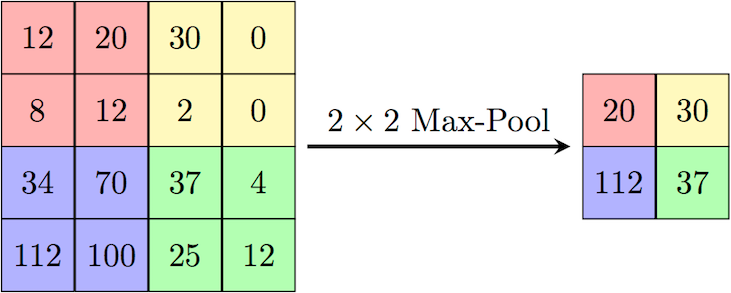
\includegraphics[width=\textwidth]{images/max_pooling_2d.png}
  \caption{Αναγωγή του Max Pooling σε δύο διαστάσεις.}
  \label{fig:max_pooling_2d}
\end{figure}

\begin{figure}[h]
  \centering
  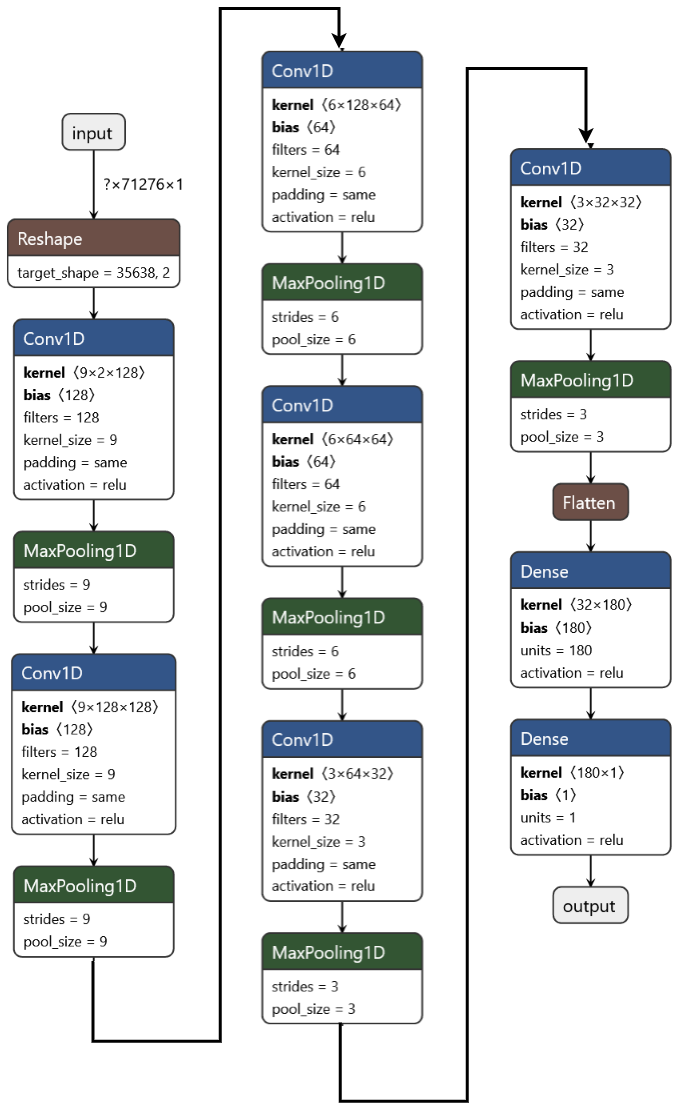
\includegraphics[width=\textwidth]{images/CNN_Arch.png}
  \caption{Η αρχιτεκτονική του μοντέλου CNN για εκτίμηση DOA.}
  \label{fig:CNN_Arch}
\end{figure}
\clearemptydoublepage

\chapter{Αποτελέσματα}\label{ch:chap4}
%!TEX root = ../main.tex
\noindent
Στις ενότητες \ref{ch:chap2} και \ref{ch:chap3}, αναλύθηκε το θεωρητικό υπόβαθρο της παρούσας εργασίας και τα τμήματα που απαρτίζουν το σύστημα εκτίμησης γωνίας άφιξης αντίστοιχα. Σε αυτό το κεφάλαιο, παρουσιάζεται η πορεία της εκπαίδευσης των νευρωνικών δικτύων καθώς και τα αποτελέσματα-προβλέψεις των μοντέλων, σε σύγκριση με άλλα ήδη υπάρχοντα μοντέλα. Παρουσιάζονται επίσης συγκριτικά τα δεδομένα που χρησιμοποιήθηκαν για την εκπαίδευση των μοντέλων, οι διαφορετικές αρχιτεκτονικές που χρησιμοποιήθηκαν καθώς και το μέγεθος των διανυσμάτων εισόδου, εφόσον αυτό είναι διαθέσιμο στην εκάστοτε εργασία.

\section{Αποτελέσματα εκπαίδευσης}
Σε αυτό το σημείο, παρουσιάζονται τα διαγράμματα που δείχνουν την πορεία εξέλιξης της τιμής των αντικειμενικών συναρτήσεων που χρησιμοποιούνται κατά την εκπαίδευση, οι οποίες είναι όπως έχει αναφερθεί το MSE, RMSE και MAE, για τα δύο διαφορετικά μοντέλα που εκπαιδεύτηκαν, το fully connected, και το convolutional.

\subsection{Πλήρως διασυνδεδεμένη αρχιτεκτονική}

Κατά την διαδικασία της εκπαίδευσης, κάθε νευρώνας εκτελεί ένα σταθμισμένο άθροισμα, το οποίο τελικά δίνεται ως είσοδος στη συνάρτηση ενεργοποίησης, ώστε να παραχθεί η έξοδος του νευρώνα. Οι πράξεις αυτές εκτελούνται γρήγορα σε σχέση με τις πράξεις που είναι απαραίτητες στις άλλες αρχιτεκτονικές, (CNN, CRNN κλπ). Στα διαγράμματα \ref{fig:FC_MSE}, \ref{fig:FC_RMSE} και \ref{fig:FC_MAE}, φαίνονται με τη σειρά η εξέλιξη των τιμών του MSE, RMSE και MAE αντίστοιχα. Τα test data χρησιμοποιούνται κατά το πέρας της εκπαίδευσης, για την τελική αξιολόγηση του μοντέλου και παρουσιάζονται σε επόμενη υποενότητα. Τα διαγράμματα αυτά περιγράφουν ουσιαστικά την \textit{ιστορία} του μοντέλου.

Το μοντέλο, ξεκινά με τελείως τυχαίες προβλέψεις, που αιτιολογούν και το εξαιρετικά μεγάλο σφάλμα κατά την αρχή της εκπαίδευσης, ενώ στη συνέχεια, \textit{μαθαίνει}, να βγάζει συμπεράσματα από τα χαρακτηριστικά των διανυσμάτων εισόδου. Με τον όρο \textit{epoch} στον άξονα \textit{Χ}, υποδηλώνεται ένα \textbf{πλήρες} πέρασμα του dataset από τον αλγόριθμο. Το μοντέλο ξεκινά να συγκλίνει περίπου μετά από 350 εποχές, όπως φαίνεται από τη συνάρτηση απώλειας MSE, όπου το σφάλμα παραμένει σχετικά σταθερό. Σε εκείνο το σημείο αξιοποιείται η τεχνική Early Stopping, όπου όταν το σφάλμα δεν μειώνεται για έναν προκαθορισμένο αριθμό εποχών, τότε τερματίζεται η διαδικασία της εκπαίδευσης για την αποφυγή σπατάλης υπολογιστικών πόρων και προφανώς, χρόνου. 

Γίνεται επίσης εμφανές, το γεγονός ότι οι καμπύλες που δείχνουν την απόδοση στα training και στα validation data απέχουν κάποια απόσταση μεταξύ τους. Αυτό είναι αναμενόμενο, και ο λόγος που η καμπύλη που αφορά τα δεδομένα εκπαίδευσης είναι πάντα κάτω από την καμπύλη του validation, είναι το γεγονός ότι τα νευρωνικά δίκτυα, και ιδιαίτερα οι fully connected αρχιτεκτονικές, έχουν την τάση να 'απομνημονεύουν' τα δεδομένα εισόδου, με αποτέλεσμα να έχουν χειρότερη απόδοση σε δεδομένα που 'βλέπουν' πρώτη φορά. Η περίπτωση στην οποία η απόσταση μεταξύ των δύο καμπυλών μεγαλώνει όσο περνάνε οι εποχές λέγεται \textbf{\textit{overfitting}} και τα επίπεδα Dropout, έχουν χρησιμοποιηθεί για την αντιμετώπισή του.

\begin{figure}[h!]
  \centering
  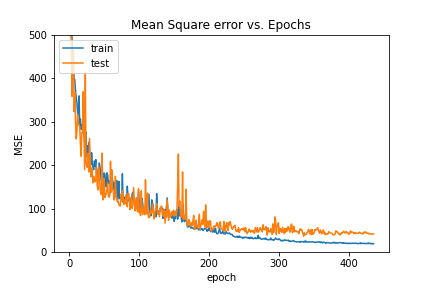
\includegraphics[width=\textwidth]{images/FC_MSE.png}
  \caption{Ιστορικό τιμών του MSE για την Fully Connected αρχιτεκτονική.}
  \label{fig:FC_MSE}
\end{figure}

\begin{figure}[h!]
  \centering
  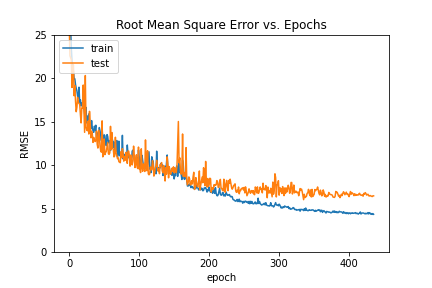
\includegraphics[width=\textwidth]{images/FC_RMSE.png}
  \caption{Ιστορικό τιμών του RMSE για την Fully Connected αρχιτεκτονική.}
  \label{fig:FC_RMSE}
\end{figure}

\begin{figure}[h!]
  \centering
  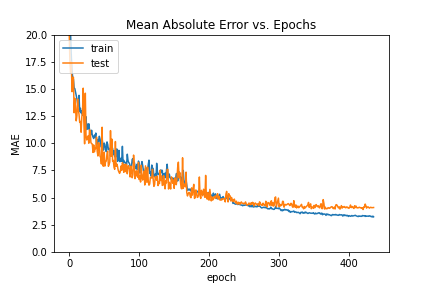
\includegraphics[width=\textwidth]{images/FC_MAE.png}
  \caption{Ιστορικό τιμών του MAE για την Fully Connected αρχιτεκτονική.}
  \label{fig:FC_MAE}
\end{figure}

\newpage
\subsection{Συνελικτική αρχιτεκτονική}

Τα αντίστοιχα αποτελέσματα για την convolutional δομή, παρουσιάζονται σε αυτή την υποενότητα, στα Σχήματα \ref{fig:CNN_MSE}, \ref{fig:CNN_RMSE} και \ref{fig:CNN_MAE} για τα MSE, RMSE και MAE αντίστοιχα. Αξίζει να σημειωθεί το γεγονός, πως το CNN, χρειάζεται τις μισές περίπου εποχές για να φτάσει στο τοπικό ελάχιστο της συνάρτησης, χωρίς αυτό να σημαίνει όμως ότι συγκλίνει γρηγορότερα από άποψη χρόνου. Η πράξη της συνέλιξης είναι ιδιαίτερα αργή από υπολογιστική άποψη, και αυτός είναι ο κυριότερος λόγος για αυτό. Παρατηρείται επίσης, πως οι καμπύλες έχουν μεγαλύτερη κλίση στην αρχή της εκπαίδευσης. 

Τα CNN είναι πιο εύρωστα στο φαινόμενο του overfitting, οπότε δεν χρειάστηκε να προστεθούν επίπεδα Dropout για την εκπαίδευση του μοντέλου. Το CNN κάνει λάθος περίπου $3.5^o$, στην πρόβλεψη της γωνίας άφιξης, δηλαδή είναι περίπου 50\% καλύτερο από την fully connected αρχιτεκτονική που έχει μέσο σφάλμα σχεδόν $6.5^o$.

\begin{figure}[h!]
  \centering
  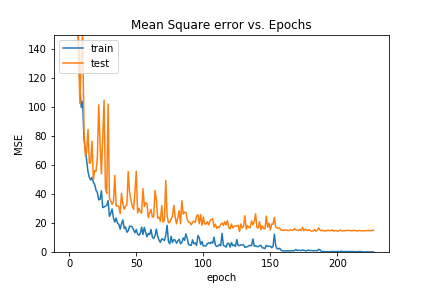
\includegraphics[width=\textwidth]{images/CNN_MSE.png}
  \caption{Ιστορικό τιμών του MSE για την συνελικτική αρχιτεκτονική.}
  \label{fig:CNN_MSE}
\end{figure}

\begin{figure}[h!]
  \centering
  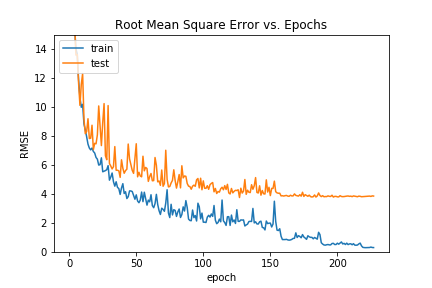
\includegraphics[width=\textwidth]{images/CNN_RMSE.png}
  \caption{Ιστορικό τιμών του RMSE για την συνελικτική αρχιτεκτονική.}
  \label{fig:CNN_RMSE}
\end{figure}

\begin{figure}[h!]
  \centering
  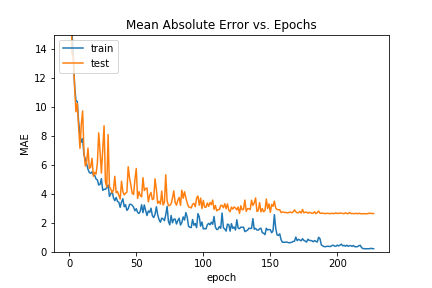
\includegraphics[width=\textwidth]{images/CNN_MAE.png}
  \caption{Ιστορικό τιμών του MAE για την Fully Connected αρχιτεκτονική.}
  \label{fig:CNN_MAE}
\end{figure}


\subsection{Χρόνοι σύγκλισης}
Εδώ παρουσιάζονται με συνοπτικό τρόπο οι χρόνοι σύγκλισης των δύο μοντέλων στον Πίνακα \ref{tab:model_times}. Σημειώνεται πως ο χρόνος που χρειάζονται και τα δύο μοντέλα για να συγκλίνουν είναι σημαντικά μικρότερος από άλλα μοντέλα που έχουν κατασκευαστεί με παρόμοιο στόχο.

\begin{table}[h!]
    \centering
    \begin{tabularx}{0.8\textwidth} { 
  | >{\centering\arraybackslash}X 
  | >{\centering\arraybackslash}X 
  | >{\centering\arraybackslash}X | }
     \hline
     Model & Epochs & Time (mins) \\[5pt]
     \hline
     Fully Connected & 436 & 125.36 \\[5pt]
    \hline
    Convolutional & 228 & 183.36 \\[5pt]
    \hline
    \end{tabularx}
    \caption{Σύγκριση χρόνων σύκλισης των μοντέλων σε εποχές και λεπτά.}
    \label{tab:model_times}
\end{table}{}

\section{Αποτελέσματα εκτίμησης}

Η απόδοση των μοντέλων αξιολογήθηκε ως προς την ικανότητά τους να εκτιμήσουν την DOA, σε δεδομένα που αντιμετωπίζουν πρώτη φορά. Αυτή ακριβώς είναι η αξία του διαχωρισμού σε train-validation-test δεδομένα, δηλαδή το ότι παρέχεται μια εγγύηση ως προς την αξιοπιστία των δεδομένων. Εκτός από τις συναρτήσεις που έχουν ήδη αναφερθεί (MSE, RMSE, MAE), χρησιμοποιούνται σε αυτό το στάδιο το \textit{Accuracy} ως προς την ταξινόμηση, των μοντέλων σε τρεις κατηγορίες προβλέψεων. Μια DOA θεωρείται σωστά ταξινομημένη εφόσον η διαφορά της προβλεπόμενης γωνίας άφιξης από την πραγματική είναι μικρότερη ή ίση με 5, 10 και 15 μοίρες για τις μετρικές Acc5, Acc10 και Acc15 αντίστοιχα. Για κάθε περιθώριο σφάλματος, το classification accuracy υπολογίζεται όπως φαίνεται στην εξίσωση \ref{eq:DOA_Accuracy}.

\begin{CEquation}
\begin{split}
    Accuracy(\%) = \frac{100}{n}\sum_{i=1}^nd_i\\
    \text{όπου } d_i = 
        \begin{cases}
         1 & \text{αν}\;|y_i-\hat{y_i}|<err\\
         0 & \text{αλλού}
         \end{cases} 
\end{split}
\label{eq:DOA_Accuracy}
\end{CEquation}

Τα αποτελέσματα των μοντέλων κατά το testing, φαίνονται στον πίνακα \ref{tab:model_accuracies}. Σημειώνεται πως τα 'Test Noise Signals' (TNS στον πίνακα) είναι τα burst θορύβου που δημιουργήθηκαν για τους σκοπούς αυτής της εργασίας. Στην περίπτωση του CNN, δοκιμάστηκε η απόδοσή του στην εκτίμηση της γωνίας άφιξης, όταν το σήμα εισόδου είναι κάτι τελείως διαφορετικό από αυτά που έχει δει στην εκπαίδευση, όπως φωνή ή μουσική. Το CNN φαίνεται πως γενικεύει εξαιρετικά σε νέα δεδομένα, επιτυγχάνοντας ένα ελάχιστο classification accuracy 79\%, και μέγιστο  85\%. 

\begin{table}[h!]
    \centering
    \begin{tabularx}{\textwidth} { 
  | >{\centering\arraybackslash}X 
  | >{\centering\arraybackslash}X 
  | >{\centering\arraybackslash}X
  | >{\centering\arraybackslash}X
  | >{\centering\arraybackslash}X
  | >{\centering\arraybackslash}X
  | >{\centering\arraybackslash}X | }
     \hline
     Dataset & MSE & RMSE & MAE & Acc5(\%) & Acc10(\%) & Acc15(\%)\\[5pt]
     \hline
     \multicolumn{7}{|c|}{Fully Connected Architecture} \\[5pt]
     \hline
     TNS & 40.5 & 6.4 & 4 & 89 & 97 & 98 \\[5pt]
     \hline
     \multicolumn{7}{|c|}{Convolutional Architecture} \\[5pt]
     \hline
     TNS & 11.3 & 3.4 & 2.3 & 96 & 99 & 100 \\[5pt]
     \hline
     Voice & 82.8 & 9.1 & 7.0 & 79 & 89 & 95 \\[5pt]
     \hline
     Bongo & 212.4 & 14.6 & 10.5 & 80 & 90 & 96 \\[5pt]
     \hline
     Cello & 123.0 & 11.1 & 9.1 & 88 & 95 & 98 \\[5pt]
     \hline
     Guitar & 130.7 & 11.4 & 9.3 & 87 & 94 & 97 \\[5pt]
     \hline
     Xyloph. & 212.4 & 14.6 & 10.5 & 80 & 90 & 96 \\[5pt]
     \hline
     CNN Mean & 128.8 & 10.7 & 8.1 & 85 & 93 & 97 \\[5pt]
     \hline
     
    \end{tabularx}
    \caption{Αποτελέσματα εκτίμισης γωνίας άφιξης για διαφορετικά σήματα διέγερσης.}
    \label{tab:model_accuracies}
\end{table}{}

Είναι εμφανές πως το CNN, έχει μακράν καλύτερα αποτελέσματα από το αντίστοιχο Fully Connected μοντέλο και για αυτόν τον λόγο κρίθηκε πως είχε νόημα να δοκιμαστεί η απόδοσή του σε διαφορετικές συνθήκες. Σημειώνεται πως οι BRIR που χρησιμοποιούνται σε αυτή την εργασία προκύπτουν από πραγματικά δωμάτια, ενώ στα περισσότερα άλλα συστήματα εντοπισμού γωνίας άφιξης, χρησιμοποιούνται συνήθως simulated δωμάτια.

\section{Σύγκριση με άλλες μεθόδους}
Η υποενότητα αυτή επικεντρώνεται στη σύγκριση της προτεινόμενης μεθόδου με άλλες δημοσιευμένες μεθόδους εκτίμησης DOA που χρησιμοποιούν τεχνικές μηχανικής μάθησης. Για το μοντέλο αυτής της εργασίας χρησιμοποιούνται οι μέσες τιμές κάθε μετρικής που προκύπτουν από εκτιμήσεις του CNN, όπως φαίνονται στον πίνακα \ref{tab:model_accuracies}, ενώ στα άλλα μοντέλα χρησιμοποιούνται τα καλύτερα αποτελέσματα που έχουν επιτευχθεί. Τονίζεται πως δεν χρησιμοποιούνται παντού οι ίδιες μετρικές, οπότε αναφέρονται όσες είναι διαθέσιμες. Σε αντίθετη περίπτωση χρησιμοποιούνται best και worst case αποτελέσματα στη θέση των Acc5 και Acc15 αντίστοιχα. Στον πίνακα \ref{tab:model_comparisons1} παρουσιάζονται οι συγκρίσεις μεταξύ των μοντέλων.

\begin{table}[h!]
    \centering
    \begin{tabularx}{\textwidth} { 
  | >{\centering\arraybackslash}X 
  | >{\centering\arraybackslash}X 
  | >{\centering\arraybackslash}X 
  | >{\centering\arraybackslash}X | }
     \hline
     Model & Acc5(\%) & Acc10(\%) & Acc15(\%) \\[5pt]
     \hline
    Proposed Model & 85 & 93 & 97 \\[5pt]
    \hline
    Intensity-CRNN (Simulated RIR) \cite{Perotin2019} & 54.3 & 94.4 & 98.9\\[5pt]
    \hline
    Intensity-CRNN (Real RIR) \cite{Perotin2019}& 26.2 & 62.6 & 78.1 \\[5pt]
    \hline
    DoaNet \cite{Perotin2019}& 59.3 & - & 95.4 \\[5pt]
    \hline
    CNN+masking \cite{Zhang2019}& 65.8 & - & 87.0 \\[5pt]
    \hline
    \end{tabularx}
    \caption{Σύγκριση DOA Accuracy της προτεινόμενης μεθόδου, με άλλες δημοσιευμένες μεθόδου.}
    \label{tab:model_comparisons1}
\end{table}{}

Για τις μεθόδους που συγκρίθηκαν στον πίνακα \ref{tab:model_comparisons1}, οι πίνακες \ref{tab:model_comparisons2} και \ref{tab:model_comparisons3} παρουσιάζουν τις διαφορετικές αρχιτεκτονικές νευρωνικών δικτύων και τα datasets που χρησιμοποιήθηκαν για την εκπαίδευσή τους. Ελέγχοντας τους δύο πίνακες ταυτόχρονα, παρατηρείται ότι η προτεινόμενη μέθοδος εξαρτάται από δεδομένα που προέρχονται από πραγματικά δωμάτια, και σε συνδυασμό με την μέθοδο \textit{profiling} που κατασκευάστηκε και αναλύθηκε στο κεφάλαιο \ref{sec:data_compression}, επιτυγχάνει εξαιρετικά αποτελέσματα ακόμα και με σχετικά μικρό dataset εκπαίδευσης. Ακόμα ένα πλεονέκτημα της προτεινόμενης μεθόδου είναι η αξιοσημείωτη ταχύτητα σύγκλισης, ολοκληρώνοντας της διαδικασία της εκπαίδευσης σε 3.5 ώρες (για το μοντέλο CNN το οποίο απαιτεί και τον περισσότερο χρόνο).

\begin{table}[h!]
    \centering
    \begin{tabularx}{\textwidth} { 
  | >{\centering\arraybackslash}X 
  | >{\centering\arraybackslash}X 
  | >{\centering\arraybackslash}X 
  | >{\centering\arraybackslash}X | }
     \hline
     Model & Architecture & R/C & NN Inputs \\[5pt]
     \hline
    Proposed Model & 1D-CNN & R & ILD+ITD Profiles \\[5pt]
    \hline
    Intensity-CRNN & 2D-CRNN & C & Acoustic Intensity Vectors\\[5pt]
    \hline
    DoaNet & 2D-CRNN & C & Magnitude + Phase Spectrograms \\[5pt]
    \hline
    CNN+masking & CRNN & C & Magnitude Spectrograms \\[5pt]
    \hline
    \end{tabularx}
    \caption{Σύγκριση των μοντέλων ως προς την αρχιτεκτονική που χρησιμοποιήθηκε και τις εισόδους. Με R/C σημειώνεται αν το νευρωνικό ήταν τύπου regression ή classification.}
    \label{tab:model_comparisons2}
\end{table}{}

\begin{table}[h!]
    \centering
    \begin{tabularx}{\textwidth} { 
  | >{\centering\arraybackslash}X 
  | >{\centering\arraybackslash}X 
  | >{\centering\arraybackslash}X 
  | >{\centering\arraybackslash}X | }
     \hline
     Model & Signals & Real Rooms & Training Vectors \\[5pt]
     \hline
    Proposed Model & Noise Burst & Yes & 6334 \\[5pt]
    \hline
    Intensity-CRNN & Bref Corpus & No & 127800 \\[5pt]
    \hline
    DoaNet & Real-life sound events & No & - \\[5pt]
    \hline
    CNN+masking & TIMIT+ChiME3 & No & 24000 \\[5pt]
    \hline
    \end{tabularx}
    \caption{Σύγκριση των μοντέλων ως προς τα δεδομένα που χρησιμοποιήθηκαν για την εκπαίδευσή τους.}
    \label{tab:model_comparisons3}
\end{table}{}

\newpage
\section{Σύγκριση αποτελεσμάτων με και χωρίς συμπίεση}

Για την επιβεβαίωση της καλής λειτουργίας του αλγορίθμου συμπίεσης, συγκρίθηκαν τα αποτελέσματα με και χωρίς τη χρήση του. Εκπαιδεύτηκαν δηλαδή μοντέλα εκ νέου, χωρίς να συμπιεστούν τα δεδομένα. Χρησιμοποιώντας στη συνέχεια τις ίδιες αρχιτεκτονικές τα μοντέλα εκπαιδεύτηκαν με τα συμπιεσμένα δεδομένα. Παρατίθενται τα αποτελέσματα του παραπάνω πειράματος, το οποίο εκτελέστηκε για fully connected και για convolutional δομές στους Πίνακες \ref{tab:model_comparisons4} και \ref{tab:model_comparisons5}.

\begin{table}[h!]
    \centering
    \begin{tabular}{|c|c|c|c|c|c|}
     \hline
     \multicolumn{6}{|c|}{Fully Connected architecture} \\[5pt]
     \hline
      & MSE & MAE & Acc5(\%) & Acc10(\%) & Time(min) \\[5pt]
     \hline
    \textbf{{\small Compressed}} & 19.9 & 3.4 & 89 & 99 & 10.93 \\[5pt]
    \hline
    {\small Uncompressed} & 49.2 & 5.3 & 83 & 96 & 41.78 \\[5pt]
    \hline
    \end{tabular}
    \caption{Σύγκριση accuracy και χρόνων στις fully connected αρχιτεκτονικές για συμπιεσμένα και ασυμπίεστα δεδομένα.}
    \label{tab:model_comparisons4}
\end{table}{}

\begin{table}[h!]
    \centering
    \begin{tabular}{|c|c|c|c|c|c|}
     \hline
     \multicolumn{6}{|c|}{Convolutional architecture} \\[5pt]
     \hline
      & MSE & MAE & Acc5(\%) & Acc10(\%) & Time(min) \\[5pt]
     \hline
    {\small Compressed} & 10.9 & 2.5 & 95 & 100 & 5.48 \\[5pt]
    \hline
    \textbf{{\small Uncompressed}} & 6.4 & 2.0 & 98 & 100 & 19.76 \\[5pt]
    \hline
    \end{tabular}
    \caption{Σύγκριση accuracy και χρόνων στις convolutional αρχιτεκτονικές για συμπιεσμένα και ασυμπίεστα δεδομένα.}
    \label{tab:model_comparisons5}
\end{table}{}

Αμέσως γίνεται εμφανές ότι και σε αυτή την περίπτωση οι συνελικτικές αρχιτεκτονικές δίνουν πολύ καλύτερα αποτελέσματα. Φαίνεται επίσης εδώ πως συγκλίνουν ταχύτερα από τις πλήρως διασυνδεδεμένες, όμως αυτό συμβαίνει διότι για να μπορέσει το μοντέλο να χωρέσει στη μνήμη περιορίστηκαν σημαντικά ο αριθμός των επιπέδων και των εκάστοτε φίλτρων σε αυτά.

Η προτεινόμενη μέθοδος συμπίεσης επιτυγχάνει ταχύτερη σύγκλιση και πολύ καλά αποτελέσματα, ακόμα και στην περίπτωση όμως που τα ασυμπίεστα δεδομένα δίνουν καλύτερα αποτελέσματα στην περίπτωση του CNN, η διαφορά είναι εξαιρετικά μικρή. Επίσης λόγω του μικρού μεγέθους των δεδομένων εισόδου, ειδικά όταν αυτά είναι συμπιεσμένα, το μοντέλο εξάγει τα αποτελέσματα σε μόλις $7msec$, μετά το στάδιο εξαγωγής των αμφιωτικών παραμέτρων.
\clearemptydoublepage

\clearemptydoublepage
%!TEX root = ../main.tex

\chapter{Συμπεράσματα}

Οι μέθοδοι για την εκτίμηση γωνίας άφιξης βασίζονται όλο και περισσότερο σε τεχνικές που χρησιμοποιούν μηχανική μάθηση, κυρίως νευρωνικά δίκτυα, που μέχρι στιγμής χρησιμοποιούν διαφορετικές προσεγγίσεις για τα δεδομένα εκπαίδευσης, τις αρχιτεκτονικές και μετρικές απόδοσης. Τέτοιες μέθοδοι συνήθως χρησιμοποιούν δεδομένα από φασματογραφήματα πλάτους ή/και φάσης.

Μια βασική απαίτηση όλων αυτών των μεθόδων είναι η αποτελεσματική χρήση των εξαχθέντων παραμέτρων από κατάλληλα σήματα, για εύρωστη και χαμηλής πολυπλοκότητας εκπαίδευση των νευρωνικών δικτύων. Τυπικά τέτοιες παράμετροι είναι οι αμφιωτικές παράμετροι ILD και ITD.

Σε αυτή την εργασία χρησιμοποιείται ένα fully connected και ένα convolutional νευρωνικό που χρησιμοποιούν μια νέα προσέγγιση για τη συμπίεση των εξαχθέντων παραμέτρων, που επιτρέπει την αποτελεσματική αναπαράστασή των ILD και ITD, για τη γρήγορη και αξιόπιστη εκπαίδευσή των μοντέλων λαμβάνοντας υπόψιν ταυτόχρονα το γεγονός ότι οι υπολογιστικοί πόροι και τα dataset είναι συνήθως περιορισμένα. Κατά την λειτουργία σε πραγματικές συνθήκες, όπως παραμέτροοι οι οποίες εξάγονται από ακουστικά σήματα που παράγονται μέσα σε δωμάτια με αντήχηση, τότε το μέγεθος των παραμέτρων καθίσταται απαγορευτικό. Με κίνητρο αυτό το γεγονός, η εργασία αυτή εισάγει μια καινούρια μέθοδο προεπεξεργασίας των αμφιωτικών παραμέτρων, η οποία απλοποιεί τα αρχικά πολυδιάστατα δεδομένα σε μόνο δύο διαστάσεις, που αποτελούν μια συνοπτική, οπτική περιγραφή τους, τα προφίλ.

Κατά τη φάση του testing, χρησιμοποιήθηκαν δεδομένα που προέρχονται από πραγματικά δωμάτια με αντήχηση και τα μοντέλα επιτυγχάνουν αποτελέσματα με υψηλή ακρίβεια, από σήματα εισόδου που είναι μόλις $200msec$. Η ακρίβεια παραμένει υψηλή ακόμα και όταν τα σήματα είναι διαφορετικά από αυτά που χρησιμοποιήθηκαν κατά την εκπαίδευση των μοντέλων.

Οι μέχρι στιγμής δοκιμές έχουν δώσει αισιόδοξα αποτελέσματα, επιβεβαιώνοντας πως η προτεινόμενη μέθοδος προσέγγισης του προβλήματος της εκτίμησης DOA, λειτουργεί ακόμα και στην περίπτωση πολύ χαμηλότερης δειγματοληψίας, όπου τα δεδομένα είναι ακόμα πιο περιορισμένα. Τα αποτελέσματα σε αυτή την περίπτωση ορισμένες φορές ξεπερνούν αυτά που έχουν παρουσιαστεί σε αυτή την εργασία.

Ο έλεγχος της απόδοσης της μεθόδου στην περίπτωση που τα δεδομένα προέρχονται από ένα δωμάτιο που δεν έχει χρησιμοποιηθεί κατά την εκπαίδευση αποτελεί αντικείμενο μελλοντικής μελέτης, όπως επίσης και η τροφοδότηση του μοντέλου με περισσότερα δωμάτια, καθώς και διαφορετικές θέσης του ακροατή μέσα σε αυτά για την επίτευξη πιο εύρωστης λειτουργίας.
\clearemptydoublepage

\listoffigures
\clearemptydoublepage
\listoftables
\clearemptydoublepage

\bibliographystyle{ieeetr}
\bibliography{thesis_bib_library}
\clearemptydoublepage

\pagestyle{empty}

\vspace*{\fill}
% \hline
\begin{flushleft}
	Πανεπιστήμιο Πατρών, Πολυτεχνική Σχολή \\
	Τμήμα Ηλεκτρολόγων Μηχανικών και Τεχνολογίας Υπολογιστών \\
	{\nomme} \\
	© \monthyear \ -- Με την επιφύλαξη παντός δικαιώματος.\\
\end{flushleft}
% \hline


\end{document}
